\documentclass{book}
\usepackage[a4paper,top=2.5cm,bottom=2.5cm,left=2.5cm,right=2.5cm]{geometry}
\usepackage{makeidx}
\usepackage{natbib}
\usepackage{graphicx}
\usepackage{multicol}
\usepackage{float}
\usepackage{listings}
\usepackage{color}
\usepackage{ifthen}
\usepackage[table]{xcolor}
\usepackage{textcomp}
\usepackage{alltt}
\usepackage{ifpdf}
\ifpdf
\usepackage[pdftex,
            pagebackref=true,
            colorlinks=true,
            linkcolor=blue,
            unicode
           ]{hyperref}
\else
\usepackage[ps2pdf,
            pagebackref=true,
            colorlinks=true,
            linkcolor=blue,
            unicode
           ]{hyperref}
\usepackage{pspicture}
\fi
\usepackage[utf8]{inputenc}
\usepackage{mathptmx}
\usepackage[scaled=.90]{helvet}
\usepackage{courier}
\usepackage{sectsty}
\usepackage{amssymb}
\usepackage[titles]{tocloft}
\usepackage{doxygen}
\lstset{language=C++,inputencoding=utf8,basicstyle=\footnotesize,breaklines=true,breakatwhitespace=true,tabsize=4,numbers=left }
\makeindex
\setcounter{tocdepth}{3}
\renewcommand{\footrulewidth}{0.4pt}
\renewcommand{\familydefault}{\sfdefault}
\hfuzz=15pt
\setlength{\emergencystretch}{15pt}
\hbadness=750
\tolerance=750
\begin{document}
\hypersetup{pageanchor=false,citecolor=blue}
\begin{titlepage}
\vspace*{7cm}
\begin{center}
{\Large Reference Manual}\\
\vspace*{1cm}
{\large Generated by Doxygen 1.8.2}\\
\vspace*{0.5cm}
{\small Fri Nov 16 2012 17:37:43}\\
\end{center}
\end{titlepage}
\clearemptydoublepage
\pagenumbering{roman}
\tableofcontents
\clearemptydoublepage
\pagenumbering{arabic}
\hypersetup{pageanchor=true,citecolor=blue}
\chapter{Hierarchical Index}
\section{Class Hierarchy}
This inheritance list is sorted roughly, but not completely, alphabetically\-:\begin{DoxyCompactList}
\item \contentsline{section}{\-\_\-\-W\-D\-I\-R}{\pageref{struct___w_d_i_r}}{}
\item \contentsline{section}{\-\_\-wdirent}{\pageref{struct__wdirent}}{}
\item \contentsline{section}{Bintree}{\pageref{class_bintree}}{}
\item \contentsline{section}{D\-I\-R}{\pageref{struct_d_i_r}}{}
\item \contentsline{section}{dirent}{\pageref{structdirent}}{}
\item \contentsline{section}{Jzon\-:\-:File\-Reader}{\pageref{class_jzon_1_1_file_reader}}{}
\item \contentsline{section}{Jzon\-:\-:File\-Writer}{\pageref{class_jzon_1_1_file_writer}}{}
\item \contentsline{section}{Jzon\-:\-:Format}{\pageref{struct_jzon_1_1_format}}{}
\item \contentsline{section}{Jzon\-:\-:Format\-Interpreter}{\pageref{class_jzon_1_1_format_interpreter}}{}
\item \contentsline{section}{Item}{\pageref{class_item}}{}
\item iterator\begin{DoxyCompactList}
\item \contentsline{section}{Jzon\-:\-:Array\-:\-:const\-\_\-iterator}{\pageref{class_jzon_1_1_array_1_1const__iterator}}{}
\item \contentsline{section}{Jzon\-:\-:Array\-:\-:iterator}{\pageref{class_jzon_1_1_array_1_1iterator}}{}
\item \contentsline{section}{Jzon\-:\-:Object\-:\-:const\-\_\-iterator}{\pageref{class_jzon_1_1_object_1_1const__iterator}}{}
\item \contentsline{section}{Jzon\-:\-:Object\-:\-:iterator}{\pageref{class_jzon_1_1_object_1_1iterator}}{}
\end{DoxyCompactList}
\item logic\-\_\-error\begin{DoxyCompactList}
\item \contentsline{section}{Jzon\-:\-:Type\-Exception}{\pageref{class_jzon_1_1_type_exception}}{}
\item \contentsline{section}{Jzon\-:\-:Value\-Exception}{\pageref{class_jzon_1_1_value_exception}}{}
\end{DoxyCompactList}
\item \contentsline{section}{Jzon\-:\-:Node}{\pageref{class_jzon_1_1_node}}{}
\begin{DoxyCompactList}
\item \contentsline{section}{Jzon\-:\-:Array}{\pageref{class_jzon_1_1_array}}{}
\item \contentsline{section}{Jzon\-:\-:Object}{\pageref{class_jzon_1_1_object}}{}
\item \contentsline{section}{Jzon\-:\-:Value}{\pageref{class_jzon_1_1_value}}{}
\end{DoxyCompactList}
\item \contentsline{section}{Orders}{\pageref{class_orders}}{}
\item out\-\_\-of\-\_\-range\begin{DoxyCompactList}
\item \contentsline{section}{Jzon\-:\-:Not\-Found\-Exception}{\pageref{class_jzon_1_1_not_found_exception}}{}
\end{DoxyCompactList}
\item \contentsline{section}{Jzon\-:\-:Parser}{\pageref{class_jzon_1_1_parser}}{}
\item \contentsline{section}{Player}{\pageref{class_player}}{}
\item \contentsline{section}{Properties}{\pageref{struct_properties}}{}
\item \contentsline{section}{Rules\-:\-:Rules\-Container}{\pageref{class_rules_1_1_rules_container}}{}
\item \contentsline{section}{Rules\-:\-:Rules\-Entry}{\pageref{class_rules_1_1_rules_entry}}{}
\item \contentsline{section}{Unit}{\pageref{class_unit}}{}
\item \contentsline{section}{Update}{\pageref{class_update}}{}
\item \contentsline{section}{Jzon\-:\-:Writer}{\pageref{class_jzon_1_1_writer}}{}
\end{DoxyCompactList}

\chapter{Class Index}
\section{Class List}
Here are the classes, structs, unions and interfaces with brief descriptions:\begin{DoxyCompactList}
\item\contentsline{section}{\hyperlink{class_matrix3}{Matrix3$<$ T $>$} (Class for matrix 3x3 )}{\pageref{class_matrix3}}{}
\item\contentsline{section}{\hyperlink{class_matrix4}{Matrix4$<$ T $>$} (Class for matrix 4x4 )}{\pageref{class_matrix4}}{}
\item\contentsline{section}{\hyperlink{class_quaternion}{Quaternion$<$ T $>$} (\hyperlink{class_quaternion}{Quaternion} class implementing some quaternion algebra operations )}{\pageref{class_quaternion}}{}
\item\contentsline{section}{\hyperlink{class_vector2}{Vector2$<$ T $>$} (Class for two dimensional vector )}{\pageref{class_vector2}}{}
\item\contentsline{section}{\hyperlink{class_vector3}{Vector3$<$ T $>$} (Class for three dimensional vector )}{\pageref{class_vector3}}{}
\item\contentsline{section}{\hyperlink{class_vector4}{Vector4$<$ T $>$} (Class for four dimensional vector )}{\pageref{class_vector4}}{}
\end{DoxyCompactList}

\chapter{File Index}
\section{File List}
Here is a list of all documented files with brief descriptions\-:\begin{DoxyCompactList}
\item\contentsline{section}{{\bfseries dirent.\-h} }{\pageref{dirent_8h}}{}
\item\contentsline{section}{{\bfseries Files.\-h} }{\pageref{_files_8h}}{}
\item\contentsline{section}{{\bfseries Jzon.\-h} }{\pageref{_jzon_8h}}{}
\item\contentsline{section}{{\bfseries Players.\-h} }{\pageref{_players_8h}}{}
\item\contentsline{section}{{\bfseries properties.\-h} }{\pageref{properties_8h}}{}
\item\contentsline{section}{\hyperlink{rules_8cpp}{rules.\-cpp} }{\pageref{rules_8cpp}}{}
\item\contentsline{section}{\hyperlink{rules_8h}{rules.\-h} }{\pageref{rules_8h}}{}
\item\contentsline{section}{{\bfseries tree.\-h} }{\pageref{tree_8h}}{}
\item\contentsline{section}{{\bfseries Units.\-h} }{\pageref{_units_8h}}{}
\item\contentsline{section}{{\bfseries Update.\-h} }{\pageref{_update_8h}}{}
\end{DoxyCompactList}

\chapter{Class Documentation}
\hypertarget{struct___w_d_i_r}{\section{\-\_\-\-W\-D\-I\-R Struct Reference}
\label{struct___w_d_i_r}\index{\-\_\-\-W\-D\-I\-R@{\-\_\-\-W\-D\-I\-R}}
}
\subsection*{Public Attributes}
\begin{DoxyCompactItemize}
\item 
\hypertarget{struct___w_d_i_r_a84ae1457352005f813ed4b3dc1994b62}{struct \hyperlink{struct__wdirent}{\-\_\-wdirent} {\bfseries ent}}\label{struct___w_d_i_r_a84ae1457352005f813ed4b3dc1994b62}

\item 
\hypertarget{struct___w_d_i_r_a2e2f2680de3f93c30245e482d2b714fa}{W\-I\-N32\-\_\-\-F\-I\-N\-D\-\_\-\-D\-A\-T\-A\-W {\bfseries find\-\_\-data}}\label{struct___w_d_i_r_a2e2f2680de3f93c30245e482d2b714fa}

\item 
\hypertarget{struct___w_d_i_r_a9b7432df163d1e291ba5925347fd4af3}{int {\bfseries cached}}\label{struct___w_d_i_r_a9b7432df163d1e291ba5925347fd4af3}

\item 
\hypertarget{struct___w_d_i_r_a694510e166fd3e797b3e15b9e4b3810a}{H\-A\-N\-D\-L\-E {\bfseries handle}}\label{struct___w_d_i_r_a694510e166fd3e797b3e15b9e4b3810a}

\item 
\hypertarget{struct___w_d_i_r_a700ff3a1096fb36452c571b0f55b4e60}{wchar\-\_\-t $\ast$ {\bfseries patt}}\label{struct___w_d_i_r_a700ff3a1096fb36452c571b0f55b4e60}

\end{DoxyCompactItemize}


The documentation for this struct was generated from the following file\-:\begin{DoxyCompactItemize}
\item 
dirent.\-h\end{DoxyCompactItemize}

\hypertarget{struct__wdirent}{\section{\-\_\-wdirent Struct Reference}
\label{struct__wdirent}\index{\-\_\-wdirent@{\-\_\-wdirent}}
}
\subsection*{Public Attributes}
\begin{DoxyCompactItemize}
\item 
\hypertarget{struct__wdirent_ac8cfaf294a0b6a49287d3f384c280c93}{long {\bfseries d\-\_\-ino}}\label{struct__wdirent_ac8cfaf294a0b6a49287d3f384c280c93}

\item 
\hypertarget{struct__wdirent_aff7f360608e576cd18cf11f2caf13ef3}{unsigned short {\bfseries d\-\_\-reclen}}\label{struct__wdirent_aff7f360608e576cd18cf11f2caf13ef3}

\item 
\hypertarget{struct__wdirent_a0050d6131e6fa90206903e216b38799e}{size\-\_\-t {\bfseries d\-\_\-namlen}}\label{struct__wdirent_a0050d6131e6fa90206903e216b38799e}

\item 
\hypertarget{struct__wdirent_a3c3874604ffccbeeaffd96709763cc3b}{int {\bfseries d\-\_\-type}}\label{struct__wdirent_a3c3874604ffccbeeaffd96709763cc3b}

\item 
\hypertarget{struct__wdirent_a5ccfbf6f19313d09437e8ee293a88385}{wchar\-\_\-t {\bfseries d\-\_\-name} \mbox{[}P\-A\-T\-H\-\_\-\-M\-A\-X+1\mbox{]}}\label{struct__wdirent_a5ccfbf6f19313d09437e8ee293a88385}

\end{DoxyCompactItemize}


The documentation for this struct was generated from the following file\-:\begin{DoxyCompactItemize}
\item 
dirent.\-h\end{DoxyCompactItemize}

\hypertarget{class_jzon_1_1_array}{\section{Jzon\-:\-:Array Class Reference}
\label{class_jzon_1_1_array}\index{Jzon\-::\-Array@{Jzon\-::\-Array}}
}
Inheritance diagram for Jzon\-:\-:Array\-:\begin{figure}[H]
\begin{center}
\leavevmode
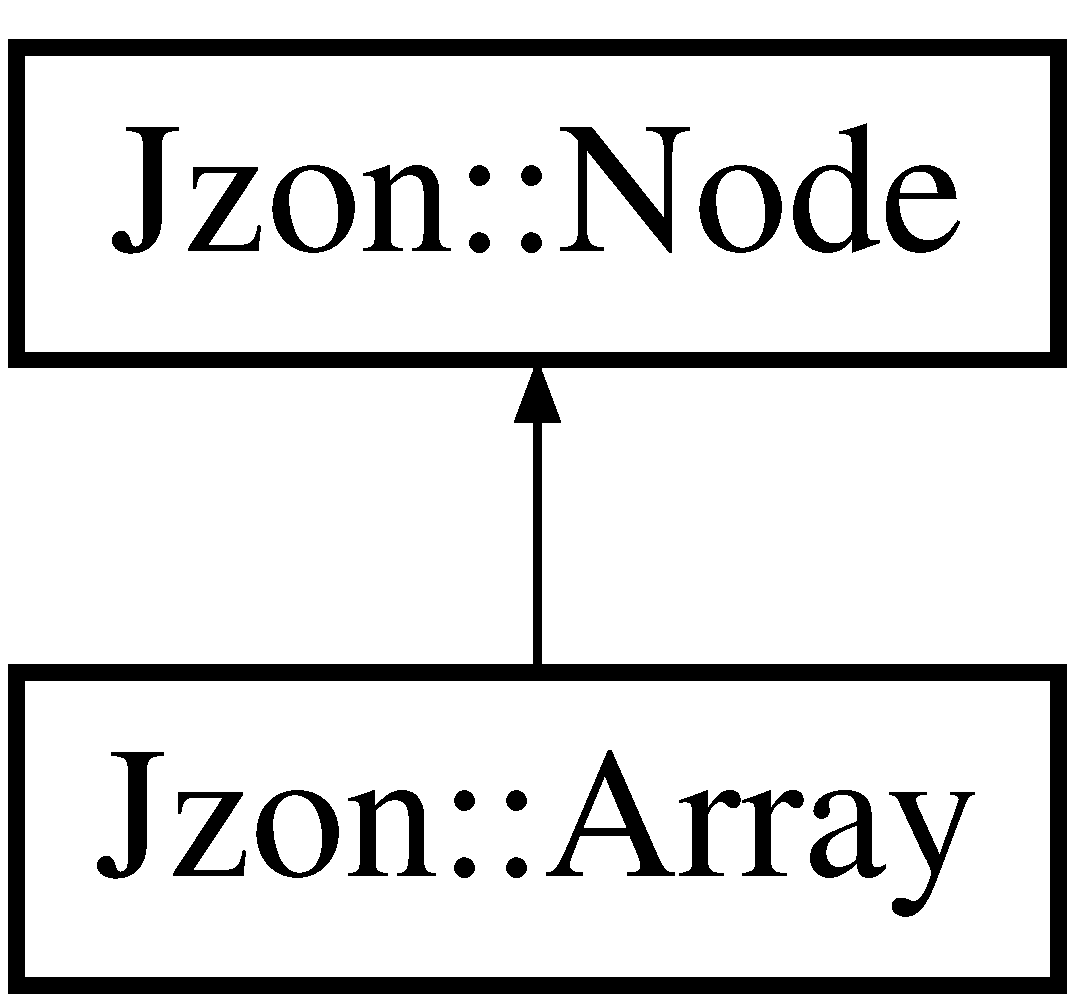
\includegraphics[height=2.000000cm]{class_jzon_1_1_array}
\end{center}
\end{figure}
\subsection*{Classes}
\begin{DoxyCompactItemize}
\item 
class \hyperlink{class_jzon_1_1_array_1_1const__iterator}{const\-\_\-iterator}
\item 
class \hyperlink{class_jzon_1_1_array_1_1iterator}{iterator}
\end{DoxyCompactItemize}
\subsection*{Public Member Functions}
\begin{DoxyCompactItemize}
\item 
\hypertarget{class_jzon_1_1_array_a289a79745f42c02471ca110bc1c603c0}{{\bfseries Array} (const \hyperlink{class_jzon_1_1_array}{Array} \&other)}\label{class_jzon_1_1_array_a289a79745f42c02471ca110bc1c603c0}

\item 
\hypertarget{class_jzon_1_1_array_a438386adb96885f30bdf7f7b223f4d79}{{\bfseries Array} (const \hyperlink{class_jzon_1_1_node}{Node} \&other)}\label{class_jzon_1_1_array_a438386adb96885f30bdf7f7b223f4d79}

\item 
\hypertarget{class_jzon_1_1_array_a4df32821b19e69448ac1f31c6278be86}{virtual Type {\bfseries Get\-Type} () const }\label{class_jzon_1_1_array_a4df32821b19e69448ac1f31c6278be86}

\item 
\hypertarget{class_jzon_1_1_array_afe136f358fe0c92269bd6b045b5dc0bc}{void {\bfseries Add} (\hyperlink{class_jzon_1_1_node}{Node} \&node)}\label{class_jzon_1_1_array_afe136f358fe0c92269bd6b045b5dc0bc}

\item 
\hypertarget{class_jzon_1_1_array_a74c5be6b360ac616631ee54f9fc47c5e}{void {\bfseries Add} (\hyperlink{class_jzon_1_1_value}{Value} node)}\label{class_jzon_1_1_array_a74c5be6b360ac616631ee54f9fc47c5e}

\item 
\hypertarget{class_jzon_1_1_array_a1fe329de43ce5ce2a9fcc8c496a2c846}{void {\bfseries Remove} (size\-\_\-t index)}\label{class_jzon_1_1_array_a1fe329de43ce5ce2a9fcc8c496a2c846}

\item 
\hypertarget{class_jzon_1_1_array_af820365490b6774d1101fc1c865fdf19}{void {\bfseries Clear} ()}\label{class_jzon_1_1_array_af820365490b6774d1101fc1c865fdf19}

\item 
\hypertarget{class_jzon_1_1_array_a4842e90116caf7d4babc81b98dcfde9c}{\hyperlink{class_jzon_1_1_array_1_1iterator}{iterator} {\bfseries begin} ()}\label{class_jzon_1_1_array_a4842e90116caf7d4babc81b98dcfde9c}

\item 
\hypertarget{class_jzon_1_1_array_ad7bccf34ce7436f396b5d714dc09c334}{\hyperlink{class_jzon_1_1_array_1_1const__iterator}{const\-\_\-iterator} {\bfseries begin} () const }\label{class_jzon_1_1_array_ad7bccf34ce7436f396b5d714dc09c334}

\item 
\hypertarget{class_jzon_1_1_array_a19fb0b40b929903bc544442c9ff1c7bc}{\hyperlink{class_jzon_1_1_array_1_1iterator}{iterator} {\bfseries end} ()}\label{class_jzon_1_1_array_a19fb0b40b929903bc544442c9ff1c7bc}

\item 
\hypertarget{class_jzon_1_1_array_a57c4259ea3192d8b25b8b6ae3a033a32}{\hyperlink{class_jzon_1_1_array_1_1const__iterator}{const\-\_\-iterator} {\bfseries end} () const }\label{class_jzon_1_1_array_a57c4259ea3192d8b25b8b6ae3a033a32}

\item 
\hypertarget{class_jzon_1_1_array_a95067395f5c19c00a02795d74ea0f1ee}{virtual size\-\_\-t {\bfseries Get\-Count} () const }\label{class_jzon_1_1_array_a95067395f5c19c00a02795d74ea0f1ee}

\item 
\hypertarget{class_jzon_1_1_array_ace64adcc3232816e3f705b74e63c4ab1}{virtual \hyperlink{class_jzon_1_1_node}{Node} \& {\bfseries Get} (size\-\_\-t index) const }\label{class_jzon_1_1_array_ace64adcc3232816e3f705b74e63c4ab1}

\end{DoxyCompactItemize}
\subsection*{Protected Member Functions}
\begin{DoxyCompactItemize}
\item 
\hypertarget{class_jzon_1_1_array_a39dc58ef32255cd8237dc726a2288fa7}{virtual \hyperlink{class_jzon_1_1_node}{Node} $\ast$ {\bfseries Get\-Copy} () const }\label{class_jzon_1_1_array_a39dc58ef32255cd8237dc726a2288fa7}

\end{DoxyCompactItemize}
\subsection*{Additional Inherited Members}


The documentation for this class was generated from the following files\-:\begin{DoxyCompactItemize}
\item 
Jzon.\-h\item 
Jzon.\-cpp\end{DoxyCompactItemize}

\hypertarget{class_bintree}{\section{Bintree Class Reference}
\label{class_bintree}\index{Bintree@{Bintree}}
}
\subsection*{Public Member Functions}
\begin{DoxyCompactItemize}
\item 
\hypertarget{class_bintree_af814eecb711f9034a4c4202597e84e19}{{\bfseries Bintree} (\hyperlink{class_item}{Item} $\ast$)}\label{class_bintree_af814eecb711f9034a4c4202597e84e19}

\item 
\hypertarget{class_bintree_a6cf7941584a9ebfcb5027a849fa72e9e}{\hyperlink{class_item}{Item} $\ast$ {\bfseries search} (unsigned long)}\label{class_bintree_a6cf7941584a9ebfcb5027a849fa72e9e}

\item 
\hypertarget{class_bintree_a1096a4a7952d52b88d8159eeaf435c0b}{void {\bfseries delete\-\_\-node} (int)}\label{class_bintree_a1096a4a7952d52b88d8159eeaf435c0b}

\item 
\hypertarget{class_bintree_ad8d4dc72e4a33b52264fc0bfb5d94b35}{void {\bfseries insert} (\hyperlink{class_item}{Item} $\ast$)}\label{class_bintree_ad8d4dc72e4a33b52264fc0bfb5d94b35}

\item 
\hypertarget{class_bintree_a78ef5e23768f407ee488341140c7a6fb}{void {\bfseries transplant} (\hyperlink{class_item}{Item} $\ast$, \hyperlink{class_item}{Item} $\ast$)}\label{class_bintree_a78ef5e23768f407ee488341140c7a6fb}

\item 
\hypertarget{class_bintree_ae92482eea09e46735f311b379b9e19cf}{\hyperlink{class_item}{Item} $\ast$ {\bfseries minimum} (\hyperlink{class_item}{Item} $\ast$)}\label{class_bintree_ae92482eea09e46735f311b379b9e19cf}

\item 
\hypertarget{class_bintree_a2d5216be079f6099a3996418cf5db1d5}{\hyperlink{class_item}{Item} $\ast$ {\bfseries get\-\_\-root} ()}\label{class_bintree_a2d5216be079f6099a3996418cf5db1d5}

\end{DoxyCompactItemize}
\subsection*{Friends}
\begin{DoxyCompactItemize}
\item 
\hypertarget{class_bintree_a2cedee6ab0da841755431efd84ad466b}{class {\bfseries Update}}\label{class_bintree_a2cedee6ab0da841755431efd84ad466b}

\end{DoxyCompactItemize}


The documentation for this class was generated from the following file\-:\begin{DoxyCompactItemize}
\item 
tree.\-h\end{DoxyCompactItemize}

\hypertarget{class_jzon_1_1_object_1_1const__iterator}{\section{Jzon\-:\-:Object\-:\-:const\-\_\-iterator Class Reference}
\label{class_jzon_1_1_object_1_1const__iterator}\index{Jzon\-::\-Object\-::const\-\_\-iterator@{Jzon\-::\-Object\-::const\-\_\-iterator}}
}
Inheritance diagram for Jzon\-:\-:Object\-:\-:const\-\_\-iterator\-:\begin{figure}[H]
\begin{center}
\leavevmode
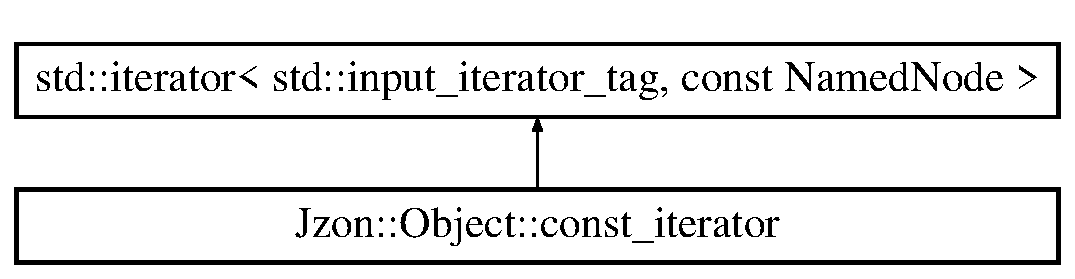
\includegraphics[height=2.000000cm]{class_jzon_1_1_object_1_1const__iterator}
\end{center}
\end{figure}
\subsection*{Public Member Functions}
\begin{DoxyCompactItemize}
\item 
\hypertarget{class_jzon_1_1_object_1_1const__iterator_ab48664cc6a72ab35fb1068771ea611c5}{{\bfseries const\-\_\-iterator} (const Named\-Node\-Ptr $\ast$o)}\label{class_jzon_1_1_object_1_1const__iterator_ab48664cc6a72ab35fb1068771ea611c5}

\item 
\hypertarget{class_jzon_1_1_object_1_1const__iterator_a9728304a0954c212eb826c184fde5803}{{\bfseries const\-\_\-iterator} (const \hyperlink{class_jzon_1_1_object_1_1const__iterator}{const\-\_\-iterator} \&it)}\label{class_jzon_1_1_object_1_1const__iterator_a9728304a0954c212eb826c184fde5803}

\item 
\hypertarget{class_jzon_1_1_object_1_1const__iterator_a9410d62280f836f64c54c5d01d889cb2}{\hyperlink{class_jzon_1_1_object_1_1const__iterator}{const\-\_\-iterator} \& {\bfseries operator++} ()}\label{class_jzon_1_1_object_1_1const__iterator_a9410d62280f836f64c54c5d01d889cb2}

\item 
\hypertarget{class_jzon_1_1_object_1_1const__iterator_a74eb2ae3261167b6c46a4d95bc252fde}{\hyperlink{class_jzon_1_1_object_1_1const__iterator}{const\-\_\-iterator} {\bfseries operator++} (int)}\label{class_jzon_1_1_object_1_1const__iterator_a74eb2ae3261167b6c46a4d95bc252fde}

\item 
\hypertarget{class_jzon_1_1_object_1_1const__iterator_a6b06d72da0f8bd3591ff695f84ab410b}{bool {\bfseries operator==} (const \hyperlink{class_jzon_1_1_object_1_1const__iterator}{const\-\_\-iterator} \&rhs)}\label{class_jzon_1_1_object_1_1const__iterator_a6b06d72da0f8bd3591ff695f84ab410b}

\item 
\hypertarget{class_jzon_1_1_object_1_1const__iterator_a5ba6a742ebf6339357b78fb925d4e97a}{bool {\bfseries operator!=} (const \hyperlink{class_jzon_1_1_object_1_1const__iterator}{const\-\_\-iterator} \&rhs)}\label{class_jzon_1_1_object_1_1const__iterator_a5ba6a742ebf6339357b78fb925d4e97a}

\item 
\hypertarget{class_jzon_1_1_object_1_1const__iterator_a46494d2e6bf4910947b8392beaf9d405}{const Named\-Node {\bfseries operator$\ast$} ()}\label{class_jzon_1_1_object_1_1const__iterator_a46494d2e6bf4910947b8392beaf9d405}

\end{DoxyCompactItemize}


The documentation for this class was generated from the following file\-:\begin{DoxyCompactItemize}
\item 
Jzon.\-h\end{DoxyCompactItemize}

\hypertarget{class_jzon_1_1_array_1_1const__iterator}{\section{Jzon\-:\-:Array\-:\-:const\-\_\-iterator Class Reference}
\label{class_jzon_1_1_array_1_1const__iterator}\index{Jzon\-::\-Array\-::const\-\_\-iterator@{Jzon\-::\-Array\-::const\-\_\-iterator}}
}
Inheritance diagram for Jzon\-:\-:Array\-:\-:const\-\_\-iterator\-:\begin{figure}[H]
\begin{center}
\leavevmode
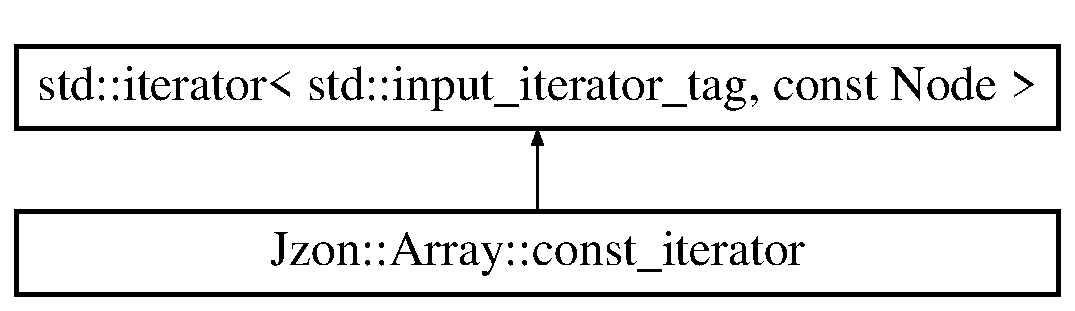
\includegraphics[height=2.000000cm]{class_jzon_1_1_array_1_1const__iterator}
\end{center}
\end{figure}
\subsection*{Public Member Functions}
\begin{DoxyCompactItemize}
\item 
\hypertarget{class_jzon_1_1_array_1_1const__iterator_a2bbffaaa14e535d421f3c4740b498e96}{{\bfseries const\-\_\-iterator} (const \hyperlink{class_jzon_1_1_node}{Node} $\ast$const $\ast$o)}\label{class_jzon_1_1_array_1_1const__iterator_a2bbffaaa14e535d421f3c4740b498e96}

\item 
\hypertarget{class_jzon_1_1_array_1_1const__iterator_a9c609e7b864892d762028bf5662e2b77}{{\bfseries const\-\_\-iterator} (const \hyperlink{class_jzon_1_1_array_1_1const__iterator}{const\-\_\-iterator} \&it)}\label{class_jzon_1_1_array_1_1const__iterator_a9c609e7b864892d762028bf5662e2b77}

\item 
\hypertarget{class_jzon_1_1_array_1_1const__iterator_a14556ac47733ee2a169723f8c5f857be}{\hyperlink{class_jzon_1_1_array_1_1const__iterator}{const\-\_\-iterator} \& {\bfseries operator++} ()}\label{class_jzon_1_1_array_1_1const__iterator_a14556ac47733ee2a169723f8c5f857be}

\item 
\hypertarget{class_jzon_1_1_array_1_1const__iterator_a8750d9d1c20a428c98a81016e4176038}{\hyperlink{class_jzon_1_1_array_1_1const__iterator}{const\-\_\-iterator} {\bfseries operator++} (int)}\label{class_jzon_1_1_array_1_1const__iterator_a8750d9d1c20a428c98a81016e4176038}

\item 
\hypertarget{class_jzon_1_1_array_1_1const__iterator_a4dfffc8199966670a94474402cf5c2b6}{bool {\bfseries operator==} (const \hyperlink{class_jzon_1_1_array_1_1const__iterator}{const\-\_\-iterator} \&rhs)}\label{class_jzon_1_1_array_1_1const__iterator_a4dfffc8199966670a94474402cf5c2b6}

\item 
\hypertarget{class_jzon_1_1_array_1_1const__iterator_afcb4d476dc47c9929ab515495dae28ad}{bool {\bfseries operator!=} (const \hyperlink{class_jzon_1_1_array_1_1const__iterator}{const\-\_\-iterator} \&rhs)}\label{class_jzon_1_1_array_1_1const__iterator_afcb4d476dc47c9929ab515495dae28ad}

\item 
\hypertarget{class_jzon_1_1_array_1_1const__iterator_a2d09cd26c9513ecc6db75acdce095e69}{const \hyperlink{class_jzon_1_1_node}{Node} \& {\bfseries operator$\ast$} ()}\label{class_jzon_1_1_array_1_1const__iterator_a2d09cd26c9513ecc6db75acdce095e69}

\end{DoxyCompactItemize}


The documentation for this class was generated from the following file\-:\begin{DoxyCompactItemize}
\item 
Jzon.\-h\end{DoxyCompactItemize}

\hypertarget{struct_d_i_r}{\section{D\-I\-R Struct Reference}
\label{struct_d_i_r}\index{D\-I\-R@{D\-I\-R}}
}
\subsection*{Public Attributes}
\begin{DoxyCompactItemize}
\item 
\hypertarget{struct_d_i_r_a59e9f5211cbb2f8e5b2807ccfdd2a7fc}{struct \hyperlink{structdirent}{dirent} {\bfseries ent}}\label{struct_d_i_r_a59e9f5211cbb2f8e5b2807ccfdd2a7fc}

\item 
\hypertarget{struct_d_i_r_a29362d4a3d7f809d0f5418b26cac5d41}{struct \hyperlink{struct___w_d_i_r}{\-\_\-\-W\-D\-I\-R} $\ast$ {\bfseries wdirp}}\label{struct_d_i_r_a29362d4a3d7f809d0f5418b26cac5d41}

\end{DoxyCompactItemize}


The documentation for this struct was generated from the following file\-:\begin{DoxyCompactItemize}
\item 
dirent.\-h\end{DoxyCompactItemize}

\hypertarget{structdirent}{\section{dirent Struct Reference}
\label{structdirent}\index{dirent@{dirent}}
}
\subsection*{Public Attributes}
\begin{DoxyCompactItemize}
\item 
\hypertarget{structdirent_acb6fecfb0e0f6fdc226dff8d56c3da4a}{long {\bfseries d\-\_\-ino}}\label{structdirent_acb6fecfb0e0f6fdc226dff8d56c3da4a}

\item 
\hypertarget{structdirent_a90dc47836e8ef510437317876368859e}{unsigned short {\bfseries d\-\_\-reclen}}\label{structdirent_a90dc47836e8ef510437317876368859e}

\item 
\hypertarget{structdirent_a09ced068b03cdb339e34840c8b709621}{size\-\_\-t {\bfseries d\-\_\-namlen}}\label{structdirent_a09ced068b03cdb339e34840c8b709621}

\item 
\hypertarget{structdirent_ad6a736cb04c7295e8f97f708324b3500}{int {\bfseries d\-\_\-type}}\label{structdirent_ad6a736cb04c7295e8f97f708324b3500}

\item 
\hypertarget{structdirent_a2db57e8744079cc6ae87dd367919957a}{char {\bfseries d\-\_\-name} \mbox{[}P\-A\-T\-H\-\_\-\-M\-A\-X+1\mbox{]}}\label{structdirent_a2db57e8744079cc6ae87dd367919957a}

\end{DoxyCompactItemize}


The documentation for this struct was generated from the following file\-:\begin{DoxyCompactItemize}
\item 
dirent.\-h\end{DoxyCompactItemize}

\hypertarget{class_jzon_1_1_file_reader}{\section{Jzon\-:\-:File\-Reader Class Reference}
\label{class_jzon_1_1_file_reader}\index{Jzon\-::\-File\-Reader@{Jzon\-::\-File\-Reader}}
}
\subsection*{Public Member Functions}
\begin{DoxyCompactItemize}
\item 
\hypertarget{class_jzon_1_1_file_reader_ad4d33b242596a91b06fdaedad8d1d347}{{\bfseries File\-Reader} (const std\-::string \&filename)}\label{class_jzon_1_1_file_reader_ad4d33b242596a91b06fdaedad8d1d347}

\item 
\hypertarget{class_jzon_1_1_file_reader_a166b5e7c68b6cd266e00980722b09885}{bool {\bfseries Read} (\hyperlink{class_jzon_1_1_node}{Node} \&node)}\label{class_jzon_1_1_file_reader_a166b5e7c68b6cd266e00980722b09885}

\item 
\hypertarget{class_jzon_1_1_file_reader_a7d2ffe10597d02fbbae2f258b05e0d79}{Node\-::\-Type {\bfseries Determine\-Type} ()}\label{class_jzon_1_1_file_reader_a7d2ffe10597d02fbbae2f258b05e0d79}

\item 
\hypertarget{class_jzon_1_1_file_reader_a1dae7fa03e20b1e4a0a0e0a306014463}{const std\-::string \& {\bfseries Get\-Error} () const }\label{class_jzon_1_1_file_reader_a1dae7fa03e20b1e4a0a0e0a306014463}

\end{DoxyCompactItemize}
\subsection*{Static Public Member Functions}
\begin{DoxyCompactItemize}
\item 
\hypertarget{class_jzon_1_1_file_reader_a8e6840bf7ade1a57f1a846c21a4c7962}{static bool {\bfseries Read\-File} (const std\-::string \&filename, \hyperlink{class_jzon_1_1_node}{Node} \&node)}\label{class_jzon_1_1_file_reader_a8e6840bf7ade1a57f1a846c21a4c7962}

\end{DoxyCompactItemize}


The documentation for this class was generated from the following files\-:\begin{DoxyCompactItemize}
\item 
Jzon.\-h\item 
Jzon.\-cpp\end{DoxyCompactItemize}

\hypertarget{class_jzon_1_1_file_writer}{\section{Jzon\-:\-:File\-Writer Class Reference}
\label{class_jzon_1_1_file_writer}\index{Jzon\-::\-File\-Writer@{Jzon\-::\-File\-Writer}}
}
\subsection*{Public Member Functions}
\begin{DoxyCompactItemize}
\item 
\hypertarget{class_jzon_1_1_file_writer_a170d50265040d8af69b56e6df9d9c9b5}{void {\bfseries Write} (const std\-::string \&filename, const \hyperlink{class_jzon_1_1_node}{Node} \&root, const \hyperlink{struct_jzon_1_1_format}{Format} \&format=No\-Format)}\label{class_jzon_1_1_file_writer_a170d50265040d8af69b56e6df9d9c9b5}

\end{DoxyCompactItemize}
\subsection*{Static Public Member Functions}
\begin{DoxyCompactItemize}
\item 
\hypertarget{class_jzon_1_1_file_writer_a328d967c23e182ed418e517c1bb15289}{static void {\bfseries Write\-File} (const std\-::string \&filename, const \hyperlink{class_jzon_1_1_node}{Node} \&root, const \hyperlink{struct_jzon_1_1_format}{Format} \&format=No\-Format)}\label{class_jzon_1_1_file_writer_a328d967c23e182ed418e517c1bb15289}

\end{DoxyCompactItemize}


The documentation for this class was generated from the following files\-:\begin{DoxyCompactItemize}
\item 
Jzon.\-h\item 
Jzon.\-cpp\end{DoxyCompactItemize}

\hypertarget{struct_jzon_1_1_format}{\section{Jzon\-:\-:Format Struct Reference}
\label{struct_jzon_1_1_format}\index{Jzon\-::\-Format@{Jzon\-::\-Format}}
}
\subsection*{Public Attributes}
\begin{DoxyCompactItemize}
\item 
\hypertarget{struct_jzon_1_1_format_a1c51a7f573ca61f17f9afa6b7e24c42a}{bool {\bfseries newline}}\label{struct_jzon_1_1_format_a1c51a7f573ca61f17f9afa6b7e24c42a}

\item 
\hypertarget{struct_jzon_1_1_format_a161944bdacf4ad60a5a5056ae70f52a5}{bool {\bfseries spacing}}\label{struct_jzon_1_1_format_a161944bdacf4ad60a5a5056ae70f52a5}

\item 
\hypertarget{struct_jzon_1_1_format_a51efdbd4255f12407ccd58218d3c10b9}{bool {\bfseries use\-Tabs}}\label{struct_jzon_1_1_format_a51efdbd4255f12407ccd58218d3c10b9}

\item 
\hypertarget{struct_jzon_1_1_format_ac95efe59857d3329bbda4925b5ad3f18}{unsigned int {\bfseries indent\-Size}}\label{struct_jzon_1_1_format_ac95efe59857d3329bbda4925b5ad3f18}

\end{DoxyCompactItemize}


The documentation for this struct was generated from the following file\-:\begin{DoxyCompactItemize}
\item 
Jzon.\-h\end{DoxyCompactItemize}

\hypertarget{class_jzon_1_1_format_interpreter}{\section{Jzon\-:\-:Format\-Interpreter Class Reference}
\label{class_jzon_1_1_format_interpreter}\index{Jzon\-::\-Format\-Interpreter@{Jzon\-::\-Format\-Interpreter}}
}
\subsection*{Public Member Functions}
\begin{DoxyCompactItemize}
\item 
\hypertarget{class_jzon_1_1_format_interpreter_a7464cb390be4ee67f45e9be26ef7ba08}{{\bfseries Format\-Interpreter} (const \hyperlink{struct_jzon_1_1_format}{Format} \&format)}\label{class_jzon_1_1_format_interpreter_a7464cb390be4ee67f45e9be26ef7ba08}

\item 
\hypertarget{class_jzon_1_1_format_interpreter_aa469372866b6e91ce2607e8bc4aea254}{void {\bfseries Set\-Format} (const \hyperlink{struct_jzon_1_1_format}{Format} \&format)}\label{class_jzon_1_1_format_interpreter_aa469372866b6e91ce2607e8bc4aea254}

\item 
\hypertarget{class_jzon_1_1_format_interpreter_a9d24644b25541b617ef5211a67d4cfc3}{std\-::string {\bfseries Get\-Indentation} (unsigned int level) const }\label{class_jzon_1_1_format_interpreter_a9d24644b25541b617ef5211a67d4cfc3}

\item 
\hypertarget{class_jzon_1_1_format_interpreter_adba21552b10df55483ae9f00704a5152}{const std\-::string \& {\bfseries Get\-Newline} () const }\label{class_jzon_1_1_format_interpreter_adba21552b10df55483ae9f00704a5152}

\item 
\hypertarget{class_jzon_1_1_format_interpreter_a8468ca011e3ad26ca9bce64542834697}{const std\-::string \& {\bfseries Get\-Spacing} () const }\label{class_jzon_1_1_format_interpreter_a8468ca011e3ad26ca9bce64542834697}

\end{DoxyCompactItemize}


The documentation for this class was generated from the following file\-:\begin{DoxyCompactItemize}
\item 
Jzon.\-cpp\end{DoxyCompactItemize}

\hypertarget{class_item}{\section{Item Class Reference}
\label{class_item}\index{Item@{Item}}
}
\subsection*{Public Member Functions}
\begin{DoxyCompactItemize}
\item 
\hypertarget{class_item_a28172fb163df01b3a78fffb0cef52da5}{{\bfseries Item} (\hyperlink{class_unit}{Unit} $\ast$)}\label{class_item_a28172fb163df01b3a78fffb0cef52da5}

\item 
\hypertarget{class_item_af1688aec8f829ebd351b47e4862f33f1}{unsigned long {\bfseries give\-\_\-key} ()}\label{class_item_af1688aec8f829ebd351b47e4862f33f1}

\item 
\hypertarget{class_item_a6bc1591d0e42a3e7a4e9af4e52bb5724}{\hyperlink{class_unit}{Unit} $\ast$ {\bfseries give\-\_\-unit} ()}\label{class_item_a6bc1591d0e42a3e7a4e9af4e52bb5724}

\end{DoxyCompactItemize}
\subsection*{Public Attributes}
\begin{DoxyCompactItemize}
\item 
\hypertarget{class_item_aed3b55d1a190f39ab686b9d6b183f20e}{\hyperlink{class_item}{Item} $\ast$ {\bfseries right}}\label{class_item_aed3b55d1a190f39ab686b9d6b183f20e}

\item 
\hypertarget{class_item_aab6663ae238e207a73baee6752fa72be}{\hyperlink{class_item}{Item} $\ast$ {\bfseries left}}\label{class_item_aab6663ae238e207a73baee6752fa72be}

\item 
\hypertarget{class_item_a5bf3ccf309da1b6f770fc9acbb6b669d}{\hyperlink{class_item}{Item} $\ast$ {\bfseries parent}}\label{class_item_a5bf3ccf309da1b6f770fc9acbb6b669d}

\end{DoxyCompactItemize}


The documentation for this class was generated from the following file\-:\begin{DoxyCompactItemize}
\item 
tree.\-h\end{DoxyCompactItemize}

\hypertarget{class_jzon_1_1_array_1_1iterator}{\section{Jzon\-:\-:Array\-:\-:iterator Class Reference}
\label{class_jzon_1_1_array_1_1iterator}\index{Jzon\-::\-Array\-::iterator@{Jzon\-::\-Array\-::iterator}}
}
Inheritance diagram for Jzon\-:\-:Array\-:\-:iterator\-:\begin{figure}[H]
\begin{center}
\leavevmode
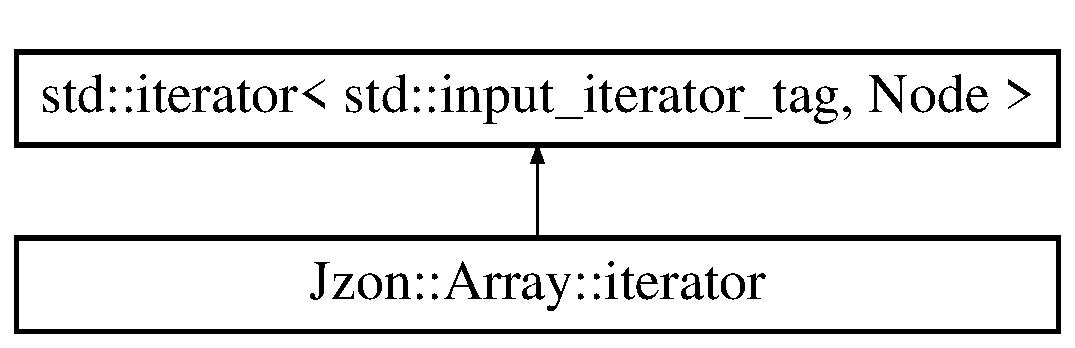
\includegraphics[height=2.000000cm]{class_jzon_1_1_array_1_1iterator}
\end{center}
\end{figure}
\subsection*{Public Member Functions}
\begin{DoxyCompactItemize}
\item 
\hypertarget{class_jzon_1_1_array_1_1iterator_abffe612d42db17d396c61b6647271630}{{\bfseries iterator} (\hyperlink{class_jzon_1_1_node}{Node} $\ast$$\ast$o)}\label{class_jzon_1_1_array_1_1iterator_abffe612d42db17d396c61b6647271630}

\item 
\hypertarget{class_jzon_1_1_array_1_1iterator_ae2871b3106d7614bd574ec052d737d5d}{{\bfseries iterator} (const \hyperlink{class_jzon_1_1_array_1_1iterator}{iterator} \&it)}\label{class_jzon_1_1_array_1_1iterator_ae2871b3106d7614bd574ec052d737d5d}

\item 
\hypertarget{class_jzon_1_1_array_1_1iterator_a74995359ea2a8af5d5363df6d4423175}{\hyperlink{class_jzon_1_1_array_1_1iterator}{iterator} \& {\bfseries operator++} ()}\label{class_jzon_1_1_array_1_1iterator_a74995359ea2a8af5d5363df6d4423175}

\item 
\hypertarget{class_jzon_1_1_array_1_1iterator_aa1c8febf6e5559f10041703ab01ce225}{\hyperlink{class_jzon_1_1_array_1_1iterator}{iterator} {\bfseries operator++} (int)}\label{class_jzon_1_1_array_1_1iterator_aa1c8febf6e5559f10041703ab01ce225}

\item 
\hypertarget{class_jzon_1_1_array_1_1iterator_a0a0d4d9a34c8c2fb9e3bad664ff54187}{bool {\bfseries operator==} (const \hyperlink{class_jzon_1_1_array_1_1iterator}{iterator} \&rhs)}\label{class_jzon_1_1_array_1_1iterator_a0a0d4d9a34c8c2fb9e3bad664ff54187}

\item 
\hypertarget{class_jzon_1_1_array_1_1iterator_abaffa19d5577aa357a69847ac5c40794}{bool {\bfseries operator!=} (const \hyperlink{class_jzon_1_1_array_1_1iterator}{iterator} \&rhs)}\label{class_jzon_1_1_array_1_1iterator_abaffa19d5577aa357a69847ac5c40794}

\item 
\hypertarget{class_jzon_1_1_array_1_1iterator_a949ae4cb25f80f5489c822a6608aa7a0}{\hyperlink{class_jzon_1_1_node}{Node} \& {\bfseries operator$\ast$} ()}\label{class_jzon_1_1_array_1_1iterator_a949ae4cb25f80f5489c822a6608aa7a0}

\end{DoxyCompactItemize}


The documentation for this class was generated from the following file\-:\begin{DoxyCompactItemize}
\item 
Jzon.\-h\end{DoxyCompactItemize}

\hypertarget{class_jzon_1_1_object_1_1iterator}{\section{Jzon\-:\-:Object\-:\-:iterator Class Reference}
\label{class_jzon_1_1_object_1_1iterator}\index{Jzon\-::\-Object\-::iterator@{Jzon\-::\-Object\-::iterator}}
}
Inheritance diagram for Jzon\-:\-:Object\-:\-:iterator\-:\begin{figure}[H]
\begin{center}
\leavevmode
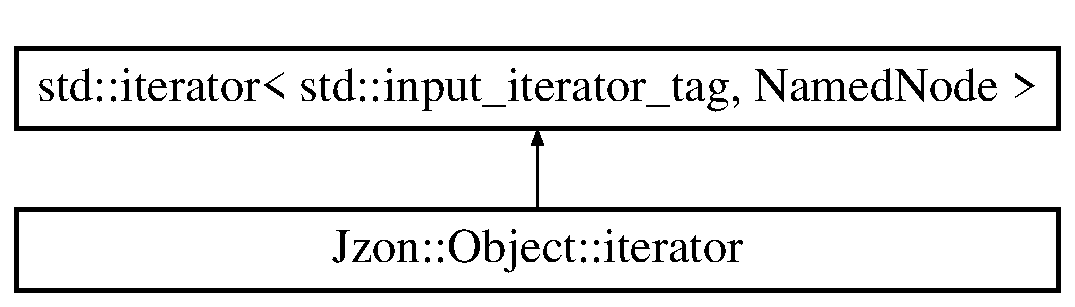
\includegraphics[height=2.000000cm]{class_jzon_1_1_object_1_1iterator}
\end{center}
\end{figure}
\subsection*{Public Member Functions}
\begin{DoxyCompactItemize}
\item 
\hypertarget{class_jzon_1_1_object_1_1iterator_ae5375ba11d0b1187146b3ac2dc74ec4c}{{\bfseries iterator} (Named\-Node\-Ptr $\ast$o)}\label{class_jzon_1_1_object_1_1iterator_ae5375ba11d0b1187146b3ac2dc74ec4c}

\item 
\hypertarget{class_jzon_1_1_object_1_1iterator_a164a528008096a59aa79b064e4b25110}{{\bfseries iterator} (const \hyperlink{class_jzon_1_1_object_1_1iterator}{iterator} \&it)}\label{class_jzon_1_1_object_1_1iterator_a164a528008096a59aa79b064e4b25110}

\item 
\hypertarget{class_jzon_1_1_object_1_1iterator_a1cc1676ac46b9d4d8cd6b2718be44d72}{\hyperlink{class_jzon_1_1_object_1_1iterator}{iterator} \& {\bfseries operator++} ()}\label{class_jzon_1_1_object_1_1iterator_a1cc1676ac46b9d4d8cd6b2718be44d72}

\item 
\hypertarget{class_jzon_1_1_object_1_1iterator_a63af275b51285d745dff3f97a0c3cd21}{\hyperlink{class_jzon_1_1_object_1_1iterator}{iterator} {\bfseries operator++} (int)}\label{class_jzon_1_1_object_1_1iterator_a63af275b51285d745dff3f97a0c3cd21}

\item 
\hypertarget{class_jzon_1_1_object_1_1iterator_a488024d8bb61e4efb256c82df4dd84bb}{bool {\bfseries operator==} (const \hyperlink{class_jzon_1_1_object_1_1iterator}{iterator} \&rhs)}\label{class_jzon_1_1_object_1_1iterator_a488024d8bb61e4efb256c82df4dd84bb}

\item 
\hypertarget{class_jzon_1_1_object_1_1iterator_a1c2f2b385ccf8f5a12890d8c43b6d742}{bool {\bfseries operator!=} (const \hyperlink{class_jzon_1_1_object_1_1iterator}{iterator} \&rhs)}\label{class_jzon_1_1_object_1_1iterator_a1c2f2b385ccf8f5a12890d8c43b6d742}

\item 
\hypertarget{class_jzon_1_1_object_1_1iterator_a8117c0c505cf83596e45e71080b71818}{Named\-Node {\bfseries operator$\ast$} ()}\label{class_jzon_1_1_object_1_1iterator_a8117c0c505cf83596e45e71080b71818}

\end{DoxyCompactItemize}


The documentation for this class was generated from the following file\-:\begin{DoxyCompactItemize}
\item 
Jzon.\-h\end{DoxyCompactItemize}

\hypertarget{class_jzon_1_1_node}{\section{Jzon\-:\-:Node Class Reference}
\label{class_jzon_1_1_node}\index{Jzon\-::\-Node@{Jzon\-::\-Node}}
}
Inheritance diagram for Jzon\-:\-:Node\-:\begin{figure}[H]
\begin{center}
\leavevmode
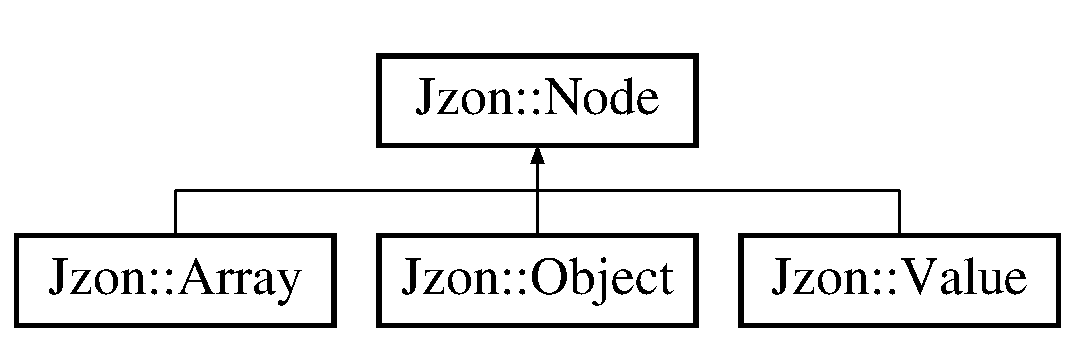
\includegraphics[height=2.000000cm]{class_jzon_1_1_node}
\end{center}
\end{figure}
\subsection*{Public Types}
\begin{DoxyCompactItemize}
\item 
enum {\bfseries Type} \{ {\bfseries T\-\_\-\-O\-B\-J\-E\-C\-T}, 
{\bfseries T\-\_\-\-A\-R\-R\-A\-Y}, 
{\bfseries T\-\_\-\-V\-A\-L\-U\-E}
 \}
\end{DoxyCompactItemize}
\subsection*{Public Member Functions}
\begin{DoxyCompactItemize}
\item 
\hypertarget{class_jzon_1_1_node_a494c21ab7856809ceea4719d6962943d}{virtual Type {\bfseries Get\-Type} () const =0}\label{class_jzon_1_1_node_a494c21ab7856809ceea4719d6962943d}

\item 
\hypertarget{class_jzon_1_1_node_a33308f53c2472c9bc49b451de67f6662}{bool {\bfseries Is\-Object} () const }\label{class_jzon_1_1_node_a33308f53c2472c9bc49b451de67f6662}

\item 
\hypertarget{class_jzon_1_1_node_a3efffe8b557ae5680ff7c64e28f8bc50}{bool {\bfseries Is\-Array} () const }\label{class_jzon_1_1_node_a3efffe8b557ae5680ff7c64e28f8bc50}

\item 
\hypertarget{class_jzon_1_1_node_aa825f03f64d58d06719a911bf9d3d489}{bool {\bfseries Is\-Value} () const }\label{class_jzon_1_1_node_aa825f03f64d58d06719a911bf9d3d489}

\item 
\hypertarget{class_jzon_1_1_node_a895d77d0c78b3e48141c3396fe4ee785}{\hyperlink{class_jzon_1_1_object}{Object} \& {\bfseries As\-Object} ()}\label{class_jzon_1_1_node_a895d77d0c78b3e48141c3396fe4ee785}

\item 
\hypertarget{class_jzon_1_1_node_a9d76906fb054e44f52d715e4191456cb}{const \hyperlink{class_jzon_1_1_object}{Object} \& {\bfseries As\-Object} () const }\label{class_jzon_1_1_node_a9d76906fb054e44f52d715e4191456cb}

\item 
\hypertarget{class_jzon_1_1_node_a055940749d53ee80b356c495f1563e06}{\hyperlink{class_jzon_1_1_array}{Array} \& {\bfseries As\-Array} ()}\label{class_jzon_1_1_node_a055940749d53ee80b356c495f1563e06}

\item 
\hypertarget{class_jzon_1_1_node_aafdde53998e10b667b29e2580913a342}{const \hyperlink{class_jzon_1_1_array}{Array} \& {\bfseries As\-Array} () const }\label{class_jzon_1_1_node_aafdde53998e10b667b29e2580913a342}

\item 
\hypertarget{class_jzon_1_1_node_a3dcc474ab6e9667f08325c953c303e61}{\hyperlink{class_jzon_1_1_value}{Value} \& {\bfseries As\-Value} ()}\label{class_jzon_1_1_node_a3dcc474ab6e9667f08325c953c303e61}

\item 
\hypertarget{class_jzon_1_1_node_a5c7a3e632bd14f910354ce1b89df1131}{const \hyperlink{class_jzon_1_1_value}{Value} \& {\bfseries As\-Value} () const }\label{class_jzon_1_1_node_a5c7a3e632bd14f910354ce1b89df1131}

\item 
\hypertarget{class_jzon_1_1_node_a0170a3faa9b165428c075e327408dce1}{virtual bool {\bfseries Is\-Null} () const }\label{class_jzon_1_1_node_a0170a3faa9b165428c075e327408dce1}

\item 
\hypertarget{class_jzon_1_1_node_a02734df98e568fae1607d870d813a805}{virtual bool {\bfseries Is\-String} () const }\label{class_jzon_1_1_node_a02734df98e568fae1607d870d813a805}

\item 
\hypertarget{class_jzon_1_1_node_a797aa0b82f01b67da6661b27d021dab5}{virtual bool {\bfseries Is\-Number} () const }\label{class_jzon_1_1_node_a797aa0b82f01b67da6661b27d021dab5}

\item 
\hypertarget{class_jzon_1_1_node_a098311227752c488d4b7917837f210b6}{virtual bool {\bfseries Is\-Bool} () const }\label{class_jzon_1_1_node_a098311227752c488d4b7917837f210b6}

\item 
\hypertarget{class_jzon_1_1_node_ac3f53a3b145697204bb1f2ccc107e5d0}{virtual std\-::string {\bfseries To\-String} () const }\label{class_jzon_1_1_node_ac3f53a3b145697204bb1f2ccc107e5d0}

\item 
\hypertarget{class_jzon_1_1_node_ae2da041c59decd652670679453451b4d}{virtual int {\bfseries To\-Int} () const }\label{class_jzon_1_1_node_ae2da041c59decd652670679453451b4d}

\item 
\hypertarget{class_jzon_1_1_node_a0a4b9b9773fd97ed03d42c84515bf2b1}{virtual float {\bfseries To\-Float} () const }\label{class_jzon_1_1_node_a0a4b9b9773fd97ed03d42c84515bf2b1}

\item 
\hypertarget{class_jzon_1_1_node_a68a8eaa99857127721e1f10f23fab85c}{virtual double {\bfseries To\-Double} () const }\label{class_jzon_1_1_node_a68a8eaa99857127721e1f10f23fab85c}

\item 
\hypertarget{class_jzon_1_1_node_a8dd81a3421dd3e8e3278c0739972249d}{virtual bool {\bfseries To\-Bool} () const }\label{class_jzon_1_1_node_a8dd81a3421dd3e8e3278c0739972249d}

\item 
\hypertarget{class_jzon_1_1_node_a33bdf9e328586d5a52ac8f86f7817134}{virtual bool {\bfseries Has} (const std\-::string \&name) const }\label{class_jzon_1_1_node_a33bdf9e328586d5a52ac8f86f7817134}

\item 
\hypertarget{class_jzon_1_1_node_a625d10ba056e724fbd3e06566d80e567}{virtual size\-\_\-t {\bfseries Get\-Count} () const }\label{class_jzon_1_1_node_a625d10ba056e724fbd3e06566d80e567}

\item 
\hypertarget{class_jzon_1_1_node_a879db6f0a36e34fe28916da41afef8c6}{virtual \hyperlink{class_jzon_1_1_node}{Node} \& {\bfseries Get} (const std\-::string \&name) const }\label{class_jzon_1_1_node_a879db6f0a36e34fe28916da41afef8c6}

\item 
\hypertarget{class_jzon_1_1_node_a3acef30b1ced9998de455a7ec4005f03}{virtual \hyperlink{class_jzon_1_1_node}{Node} \& {\bfseries Get} (size\-\_\-t index) const }\label{class_jzon_1_1_node_a3acef30b1ced9998de455a7ec4005f03}

\end{DoxyCompactItemize}
\subsection*{Static Public Member Functions}
\begin{DoxyCompactItemize}
\item 
\hypertarget{class_jzon_1_1_node_afcdb671ccea4b131592a393af3b1a250}{static Type {\bfseries Determine\-Type} (const std\-::string \&json)}\label{class_jzon_1_1_node_afcdb671ccea4b131592a393af3b1a250}

\end{DoxyCompactItemize}
\subsection*{Protected Member Functions}
\begin{DoxyCompactItemize}
\item 
\hypertarget{class_jzon_1_1_node_ac396a4b711b5731ecf26728a78af72fd}{virtual \hyperlink{class_jzon_1_1_node}{Node} $\ast$ {\bfseries Get\-Copy} () const =0}\label{class_jzon_1_1_node_ac396a4b711b5731ecf26728a78af72fd}

\end{DoxyCompactItemize}
\subsection*{Friends}
\begin{DoxyCompactItemize}
\item 
\hypertarget{class_jzon_1_1_node_a0720b5f434e636e22a3ed34f847eec57}{class {\bfseries Object}}\label{class_jzon_1_1_node_a0720b5f434e636e22a3ed34f847eec57}

\item 
\hypertarget{class_jzon_1_1_node_ae5050cd67e450419cf638e2a09bf11c9}{class {\bfseries Array}}\label{class_jzon_1_1_node_ae5050cd67e450419cf638e2a09bf11c9}

\end{DoxyCompactItemize}


The documentation for this class was generated from the following files\-:\begin{DoxyCompactItemize}
\item 
Jzon.\-h\item 
Jzon.\-cpp\end{DoxyCompactItemize}

\hypertarget{class_jzon_1_1_not_found_exception}{\section{Jzon\-:\-:Not\-Found\-Exception Class Reference}
\label{class_jzon_1_1_not_found_exception}\index{Jzon\-::\-Not\-Found\-Exception@{Jzon\-::\-Not\-Found\-Exception}}
}
Inheritance diagram for Jzon\-:\-:Not\-Found\-Exception\-:\begin{figure}[H]
\begin{center}
\leavevmode
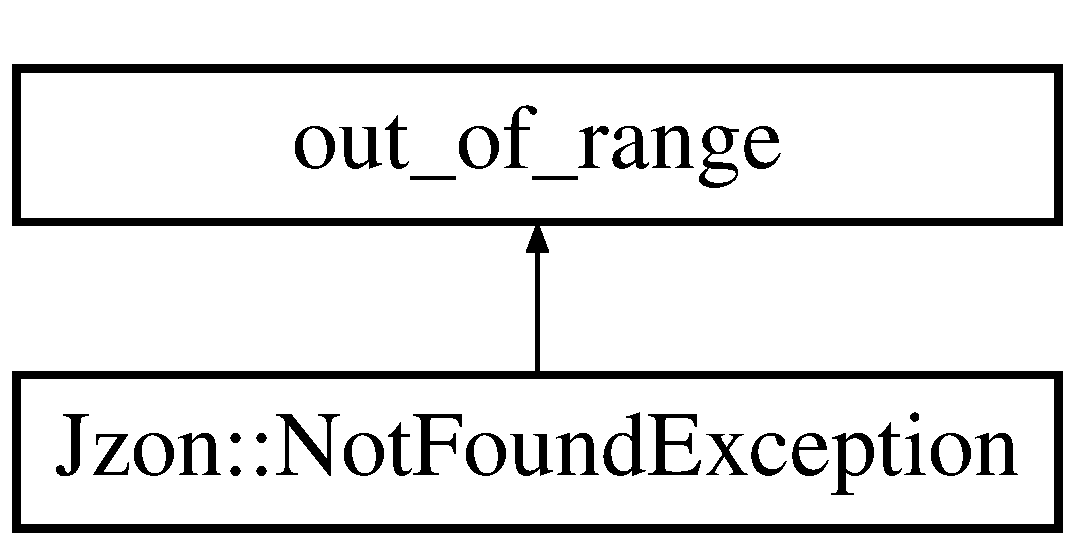
\includegraphics[height=2.000000cm]{class_jzon_1_1_not_found_exception}
\end{center}
\end{figure}


The documentation for this class was generated from the following file\-:\begin{DoxyCompactItemize}
\item 
Jzon.\-h\end{DoxyCompactItemize}

\hypertarget{class_jzon_1_1_object}{\section{Jzon\-:\-:Object Class Reference}
\label{class_jzon_1_1_object}\index{Jzon\-::\-Object@{Jzon\-::\-Object}}
}
Inheritance diagram for Jzon\-:\-:Object\-:\begin{figure}[H]
\begin{center}
\leavevmode
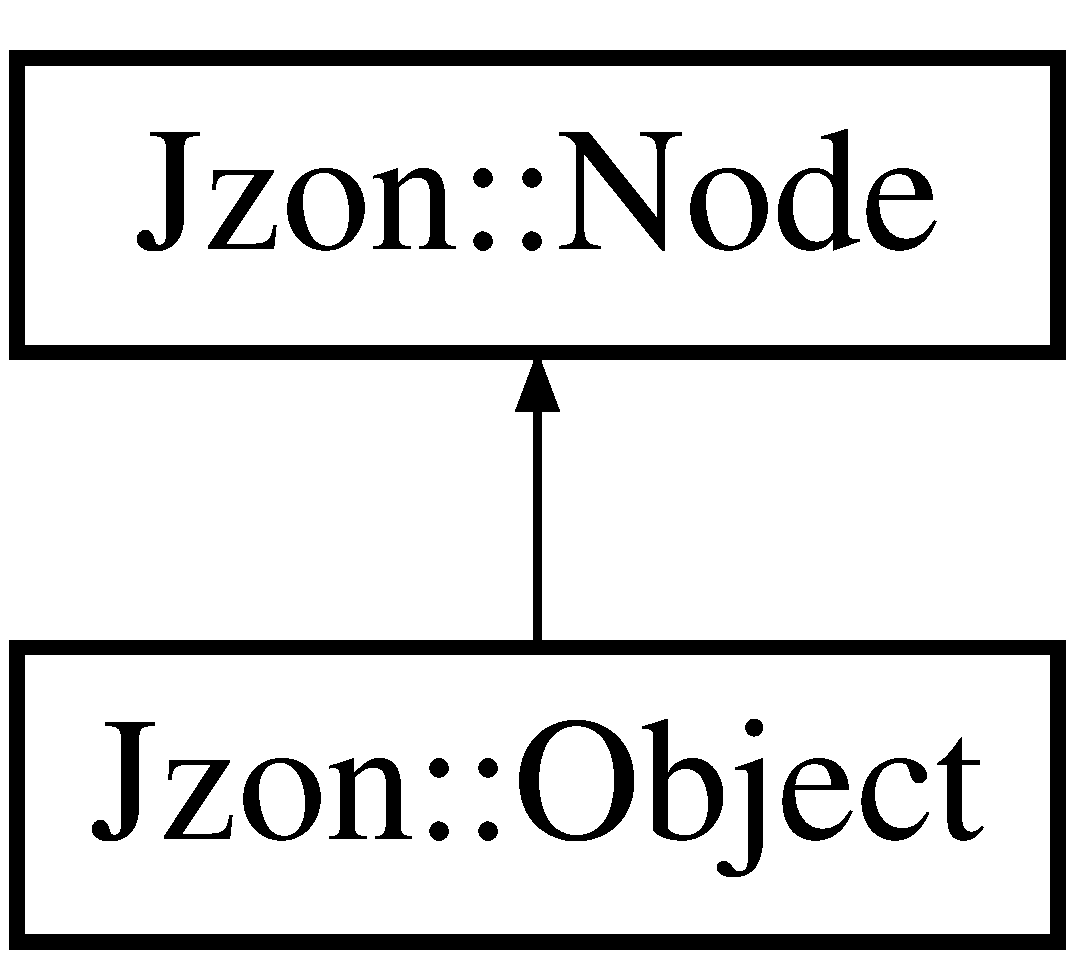
\includegraphics[height=2.000000cm]{class_jzon_1_1_object}
\end{center}
\end{figure}
\subsection*{Classes}
\begin{DoxyCompactItemize}
\item 
class \hyperlink{class_jzon_1_1_object_1_1const__iterator}{const\-\_\-iterator}
\item 
class \hyperlink{class_jzon_1_1_object_1_1iterator}{iterator}
\end{DoxyCompactItemize}
\subsection*{Public Member Functions}
\begin{DoxyCompactItemize}
\item 
\hypertarget{class_jzon_1_1_object_adb1d5cf3f312c34bece55036e48f9f35}{{\bfseries Object} (const \hyperlink{class_jzon_1_1_object}{Object} \&other)}\label{class_jzon_1_1_object_adb1d5cf3f312c34bece55036e48f9f35}

\item 
\hypertarget{class_jzon_1_1_object_a37034187776cfae7c9be8e26b1c0be33}{{\bfseries Object} (const \hyperlink{class_jzon_1_1_node}{Node} \&other)}\label{class_jzon_1_1_object_a37034187776cfae7c9be8e26b1c0be33}

\item 
\hypertarget{class_jzon_1_1_object_abbce4e6637e62a3264896e8ecf3fdddc}{virtual Type {\bfseries Get\-Type} () const }\label{class_jzon_1_1_object_abbce4e6637e62a3264896e8ecf3fdddc}

\item 
\hypertarget{class_jzon_1_1_object_a62048e8fdb5348a7899bb9b2dfd7628c}{void {\bfseries Add} (const std\-::string \&name, \hyperlink{class_jzon_1_1_node}{Node} \&node)}\label{class_jzon_1_1_object_a62048e8fdb5348a7899bb9b2dfd7628c}

\item 
\hypertarget{class_jzon_1_1_object_af353b25b1d3c157c88c01595d8e5bca3}{void {\bfseries Add} (const std\-::string \&name, \hyperlink{class_jzon_1_1_value}{Value} node)}\label{class_jzon_1_1_object_af353b25b1d3c157c88c01595d8e5bca3}

\item 
\hypertarget{class_jzon_1_1_object_a8f28bd22e6e1db9d467f1be1f61a5832}{void {\bfseries Remove} (const std\-::string \&name)}\label{class_jzon_1_1_object_a8f28bd22e6e1db9d467f1be1f61a5832}

\item 
\hypertarget{class_jzon_1_1_object_a0a2ad1f23d5c49aaeff4f28fa17e143f}{void {\bfseries Clear} ()}\label{class_jzon_1_1_object_a0a2ad1f23d5c49aaeff4f28fa17e143f}

\item 
\hypertarget{class_jzon_1_1_object_a8019eb473c3c08bba82ba0569141fea7}{\hyperlink{class_jzon_1_1_object_1_1iterator}{iterator} {\bfseries begin} ()}\label{class_jzon_1_1_object_a8019eb473c3c08bba82ba0569141fea7}

\item 
\hypertarget{class_jzon_1_1_object_a8c58b2af4344c07a8b8048c0bc271838}{\hyperlink{class_jzon_1_1_object_1_1const__iterator}{const\-\_\-iterator} {\bfseries begin} () const }\label{class_jzon_1_1_object_a8c58b2af4344c07a8b8048c0bc271838}

\item 
\hypertarget{class_jzon_1_1_object_a294ecc467022f720e7377a0a509738bb}{\hyperlink{class_jzon_1_1_object_1_1iterator}{iterator} {\bfseries end} ()}\label{class_jzon_1_1_object_a294ecc467022f720e7377a0a509738bb}

\item 
\hypertarget{class_jzon_1_1_object_a44077e96e885dc470ba5eed7356be42a}{\hyperlink{class_jzon_1_1_object_1_1const__iterator}{const\-\_\-iterator} {\bfseries end} () const }\label{class_jzon_1_1_object_a44077e96e885dc470ba5eed7356be42a}

\item 
\hypertarget{class_jzon_1_1_object_aaf903fd38759cda5c1aa7e626ac8015b}{virtual bool {\bfseries Has} (const std\-::string \&name) const }\label{class_jzon_1_1_object_aaf903fd38759cda5c1aa7e626ac8015b}

\item 
\hypertarget{class_jzon_1_1_object_a5d5ce0af633ace9dbab2fbf41ff9cba5}{virtual size\-\_\-t {\bfseries Get\-Count} () const }\label{class_jzon_1_1_object_a5d5ce0af633ace9dbab2fbf41ff9cba5}

\item 
\hypertarget{class_jzon_1_1_object_aa040339365c26fc93ade6258ba31b6c0}{virtual \hyperlink{class_jzon_1_1_node}{Node} \& {\bfseries Get} (const std\-::string \&name) const }\label{class_jzon_1_1_object_aa040339365c26fc93ade6258ba31b6c0}

\end{DoxyCompactItemize}
\subsection*{Protected Member Functions}
\begin{DoxyCompactItemize}
\item 
\hypertarget{class_jzon_1_1_object_a7eb4ae002d0a4295d365eec168ff07da}{virtual \hyperlink{class_jzon_1_1_node}{Node} $\ast$ {\bfseries Get\-Copy} () const }\label{class_jzon_1_1_object_a7eb4ae002d0a4295d365eec168ff07da}

\end{DoxyCompactItemize}
\subsection*{Additional Inherited Members}


The documentation for this class was generated from the following files\-:\begin{DoxyCompactItemize}
\item 
Jzon.\-h\item 
Jzon.\-cpp\end{DoxyCompactItemize}

\hypertarget{class_orders}{\section{Orders Class Reference}
\label{class_orders}\index{Orders@{Orders}}
}
\subsection*{Public Member Functions}
\begin{DoxyCompactItemize}
\item 
\hypertarget{class_orders_a2b142a6720700b6e0f39b804c0e838a4}{void {\bfseries name\-And\-Time\-Stamp} (string)}\label{class_orders_a2b142a6720700b6e0f39b804c0e838a4}

\item 
\hypertarget{class_orders_abcb5d4cb35dc745ab33438a90e283aff}{void {\bfseries get\-\_\-units} (\hyperlink{class_jzon_1_1_node}{Node} \&, Info $\ast$)}\label{class_orders_abcb5d4cb35dc745ab33438a90e283aff}

\item 
\hypertarget{class_orders_a03971ccf1fa121eb1a8bb5d59872334d}{void {\bfseries get\-\_\-targetids} (\hyperlink{class_jzon_1_1_node}{Node} \&, Info $\ast$)}\label{class_orders_a03971ccf1fa121eb1a8bb5d59872334d}

\item 
\hypertarget{class_orders_a7c5875d9544aab63973510beda5c5282}{void {\bfseries get\-\_\-coordinates} (\hyperlink{class_jzon_1_1_node}{Node} \&, Info $\ast$)}\label{class_orders_a7c5875d9544aab63973510beda5c5282}

\item 
\hypertarget{class_orders_a85e506850d29bc4330b6716b3e175472}{void {\bfseries get\-\_\-buys} (\hyperlink{class_jzon_1_1_node}{Node} \&)}\label{class_orders_a85e506850d29bc4330b6716b3e175472}

\item 
\hypertarget{class_orders_ae1d3763c5006288cb9f261d7f446ae19}{void {\bfseries get\-\_\-messages} (\hyperlink{class_jzon_1_1_node}{Node} \&)}\label{class_orders_ae1d3763c5006288cb9f261d7f446ae19}

\item 
\hypertarget{class_orders_a91f87f34c7d647136392804de2834886}{void {\bfseries get\-\_\-specials} (\hyperlink{class_jzon_1_1_node}{Node} \&)}\label{class_orders_a91f87f34c7d647136392804de2834886}

\item 
\hypertarget{class_orders_a994526424a9d9731e94a59d07696e6bd}{void {\bfseries get\-\_\-drops} (\hyperlink{class_jzon_1_1_node}{Node} \&)}\label{class_orders_a994526424a9d9731e94a59d07696e6bd}

\end{DoxyCompactItemize}
\subsection*{Friends}
\begin{DoxyCompactItemize}
\item 
\hypertarget{class_orders_a2cedee6ab0da841755431efd84ad466b}{class {\bfseries Update}}\label{class_orders_a2cedee6ab0da841755431efd84ad466b}

\item 
\hypertarget{class_orders_a7d948f67d6567290a086da4d251348e6}{void {\bfseries name\-And\-Time\-Stamp} (string, \hyperlink{class_orders}{Orders} \&)}\label{class_orders_a7d948f67d6567290a086da4d251348e6}

\item 
\hypertarget{class_orders_a0f5c5536c83e028fc92b96d122a4a091}{\hyperlink{class_orders}{Orders} {\bfseries jzon\-\_\-get} (\hyperlink{class_jzon_1_1_object}{Object}, string)}\label{class_orders_a0f5c5536c83e028fc92b96d122a4a091}

\item 
\hypertarget{class_orders_a6c4e48d52301cb2e2ee86c2814a4108e}{queue$<$ \hyperlink{class_orders}{Orders} $>$ {\bfseries get\-\_\-files} ()}\label{class_orders_a6c4e48d52301cb2e2ee86c2814a4108e}

\end{DoxyCompactItemize}


The documentation for this class was generated from the following file\-:\begin{DoxyCompactItemize}
\item 
Files.\-h\end{DoxyCompactItemize}

\hypertarget{class_jzon_1_1_parser}{\section{Jzon\-:\-:Parser Class Reference}
\label{class_jzon_1_1_parser}\index{Jzon\-::\-Parser@{Jzon\-::\-Parser}}
}
\subsection*{Public Member Functions}
\begin{DoxyCompactItemize}
\item 
\hypertarget{class_jzon_1_1_parser_ae6e5c8815bf569f85afc7aa974be185c}{{\bfseries Parser} (\hyperlink{class_jzon_1_1_node}{Node} \&root)}\label{class_jzon_1_1_parser_ae6e5c8815bf569f85afc7aa974be185c}

\item 
\hypertarget{class_jzon_1_1_parser_aa4db81087c1000c4d7cba127405fd12d}{{\bfseries Parser} (\hyperlink{class_jzon_1_1_node}{Node} \&root, const std\-::string \&json)}\label{class_jzon_1_1_parser_aa4db81087c1000c4d7cba127405fd12d}

\item 
\hypertarget{class_jzon_1_1_parser_a13811b1efc16acf444a9ae41bdc84eed}{void {\bfseries Set\-Json} (const std\-::string \&json)}\label{class_jzon_1_1_parser_a13811b1efc16acf444a9ae41bdc84eed}

\item 
\hypertarget{class_jzon_1_1_parser_ac0897dfcf6f0f5ec1605564b9064c3fe}{bool {\bfseries Parse} ()}\label{class_jzon_1_1_parser_ac0897dfcf6f0f5ec1605564b9064c3fe}

\item 
\hypertarget{class_jzon_1_1_parser_a15f064f5f56458a205f67fae85ac6955}{const std\-::string \& {\bfseries Get\-Error} () const }\label{class_jzon_1_1_parser_a15f064f5f56458a205f67fae85ac6955}

\end{DoxyCompactItemize}


The documentation for this class was generated from the following files\-:\begin{DoxyCompactItemize}
\item 
Jzon.\-h\item 
Jzon.\-cpp\end{DoxyCompactItemize}

\hypertarget{class_player}{\section{Player Class Reference}
\label{class_player}\index{Player@{Player}}
}
\subsection*{Public Member Functions}
\begin{DoxyCompactItemize}
\item 
\hypertarget{class_player_aaf1dcc6f6b07ba59fbbeb89f926cd0da}{{\bfseries Player} (string, int)}\label{class_player_aaf1dcc6f6b07ba59fbbeb89f926cd0da}

\item 
\hypertarget{class_player_afca8141f38b60b526fd2f874523a2726}{string {\bfseries get\-\_\-name} ()}\label{class_player_afca8141f38b60b526fd2f874523a2726}

\item 
\hypertarget{class_player_aec2430eb4f755d97e4a314f425e2d675}{int {\bfseries get\-\_\-balance} ()}\label{class_player_aec2430eb4f755d97e4a314f425e2d675}

\item 
\hypertarget{class_player_af0435bc3b2479970baa6e68b357413fe}{void {\bfseries sub\-\_\-balance} (int cost)}\label{class_player_af0435bc3b2479970baa6e68b357413fe}

\item 
\hypertarget{class_player_a93a82d102daa721442afb04d3e15bf94}{bool {\bfseries has\-\_\-enough\-\_\-money} (unsigned int)}\label{class_player_a93a82d102daa721442afb04d3e15bf94}

\end{DoxyCompactItemize}


The documentation for this class was generated from the following file\-:\begin{DoxyCompactItemize}
\item 
Players.\-h\end{DoxyCompactItemize}

\hypertarget{struct_properties}{\section{Properties Struct Reference}
\label{struct_properties}\index{Properties@{Properties}}
}
\subsection*{Public Attributes}
\begin{DoxyCompactItemize}
\item 
\hypertarget{struct_properties_af81893ae10c90800cc9e9cc7c4584c8b}{int {\bfseries tick\-\_\-size}}\label{struct_properties_af81893ae10c90800cc9e9cc7c4584c8b}

\item 
\hypertarget{struct_properties_af8029e79aa7ccd6a80ceed9ac2277bca}{bool {\bfseries keep\-\_\-orders}}\label{struct_properties_af8029e79aa7ccd6a80ceed9ac2277bca}

\item 
\hypertarget{struct_properties_a4bd2b7c4046e11a6780de734dbd08e30}{string {\bfseries servername}}\label{struct_properties_a4bd2b7c4046e11a6780de734dbd08e30}

\item 
\hypertarget{struct_properties_ae358832dbf2b9b88d210d63e53100dd8}{int {\bfseries player\-\_\-count}}\label{struct_properties_ae358832dbf2b9b88d210d63e53100dd8}

\item 
\hypertarget{struct_properties_a682adde77037f30608f504369ff5ab81}{int {\bfseries balance}}\label{struct_properties_a682adde77037f30608f504369ff5ab81}

\item 
\hypertarget{struct_properties_ab98bca3e274ed9e6e10a5b6b64208836}{string {\bfseries rules}}\label{struct_properties_ab98bca3e274ed9e6e10a5b6b64208836}

\end{DoxyCompactItemize}


The documentation for this struct was generated from the following file\-:\begin{DoxyCompactItemize}
\item 
properties.\-h\end{DoxyCompactItemize}

\hypertarget{class_rules_1_1_rules_container}{\section{Rules\-:\-:Rules\-Container Class Reference}
\label{class_rules_1_1_rules_container}\index{Rules\-::\-Rules\-Container@{Rules\-::\-Rules\-Container}}
}


Parent container for game rules.  




{\ttfamily \#include $<$rules.\-h$>$}

\subsection*{Public Member Functions}
\begin{DoxyCompactItemize}
\item 
\hyperlink{class_rules_1_1_rules_entry}{Rules\-Entry} $\ast$ \hyperlink{class_rules_1_1_rules_container_a53aecfc2e5e4608210a3aa1a42a06733}{get\-Entry} (string group\-Key, string entry\-Key)
\begin{DoxyCompactList}\small\item\em Retrieves a \hyperlink{class_rules_1_1_rules_entry}{Rules\-Entry} class within. \end{DoxyCompactList}\item 
set$<$ string $>$ \hyperlink{class_rules_1_1_rules_container_af7d4181a8517b91c7ef647ae86fabd59}{get\-Single\-Entry\-Keys} ()
\item 
set$<$ string $>$ \hyperlink{class_rules_1_1_rules_container_ac50d947a7f420cc56eb1c675800af601}{get\-Group\-Entry\-Keys} (string group\-Key)
\item 
set$<$ string $>$ \hyperlink{class_rules_1_1_rules_container_ad2abd5e08329b09ade41a94522d5a422}{get\-Group\-Keys} ()
\item 
bool \hyperlink{class_rules_1_1_rules_container_a38996e8fcd4bb07301c47e8dd0fb8685}{rm\-Entry} (string group\-Key, string entry\-Key)
\begin{DoxyCompactList}\small\item\em Removes an entry. Also removes newly-\/empty groups. \end{DoxyCompactList}\item 
string \hyperlink{class_rules_1_1_rules_container_a933f0a5e2471bb618c00fb1a1986e6e5}{serialize} ()
\begin{DoxyCompactList}\small\item\em Serializes all member \hyperlink{class_rules_1_1_rules_entry}{Rules\-Entry} classes in one big J\-S\-O\-N string. \end{DoxyCompactList}\item 
double \hyperlink{class_rules_1_1_rules_container_a6e0dbfc0c46ffb0a9556623723c54597}{get\-Double} (string group\-Key, string entry\-Key, string value\-Key)
\begin{DoxyCompactList}\small\item\em Gets a double value from a grouped or single rules entry. \end{DoxyCompactList}\item 
double \hyperlink{class_rules_1_1_rules_container_aea3e4ac2297f82cf34f4fdbc1d1a50e9}{get\-Double} (string entry\-Key, string value\-Key)
\begin{DoxyCompactList}\small\item\em Gets a double value from a single rules entry only. \end{DoxyCompactList}\item 
void \hyperlink{class_rules_1_1_rules_container_afd09a98cb51bfa71ec6f1107878d7568}{add\-Double} (double value, string group\-Key, string entry\-Key, string value\-Key)
\begin{DoxyCompactList}\small\item\em Adds a double record. Will automatically create groups and entries as needed. \end{DoxyCompactList}\item 
vector$<$ double $>$ \hyperlink{class_rules_1_1_rules_container_a3a63291a418002e075fd5bbf3370c0d8}{get\-Double\-Array} (string group\-Key, string entry\-Key, string value\-Key)
\begin{DoxyCompactList}\small\item\em Gets a double array (S\-T\-L vector) value from a grouped or single rules entry. \end{DoxyCompactList}\item 
vector$<$ double $>$ \hyperlink{class_rules_1_1_rules_container_af366a4e784f723be54d2f5da301f59ff}{get\-Double\-Array} (string entry\-Key, string value\-Key)
\begin{DoxyCompactList}\small\item\em Gets a double array (S\-T\-L vector) value from a single rules entry only. \end{DoxyCompactList}\item 
void \hyperlink{class_rules_1_1_rules_container_acf6173b4cfef7a9aaa04ac27c4782007}{add\-Double\-Array} (vector$<$ double $>$ value, string group\-Key, string entry\-Key, string value\-Key)
\begin{DoxyCompactList}\small\item\em Adds a double array (S\-T\-L vector) record. Will automatically create groups and entries as needed. \end{DoxyCompactList}\item 
string \hyperlink{class_rules_1_1_rules_container_ad8a93e5441719e6f52239cc56500eb3f}{get\-String} (string group\-Key, string entry\-Key, string value\-Key)
\begin{DoxyCompactList}\small\item\em Gets a string value from a grouped or single rules entry. \end{DoxyCompactList}\item 
string \hyperlink{class_rules_1_1_rules_container_affcb0dcb03e673c44a04baffa470edbf}{get\-String} (string entry\-Key, string value\-Key)
\begin{DoxyCompactList}\small\item\em Gets a string value from a single rules entry only. \end{DoxyCompactList}\item 
void \hyperlink{class_rules_1_1_rules_container_abf95f3b2bbd9133c24994b8c4bb656b0}{add\-String} (string value, string group\-Key, string entry\-Key, string value\-Key)
\begin{DoxyCompactList}\small\item\em Adds a string record. Will automatically create groups and entries as needed. \end{DoxyCompactList}\item 
vector$<$ string $>$ \hyperlink{class_rules_1_1_rules_container_aded0080ba412463b5bc6c19e6699292a}{get\-String\-Array} (string group\-Key, string entry\-Key, string value\-Key)
\begin{DoxyCompactList}\small\item\em Gets a string array (S\-T\-L vector) value from a grouped or single rules entry. \end{DoxyCompactList}\item 
vector$<$ string $>$ \hyperlink{class_rules_1_1_rules_container_a6d1fc8b4284cec7f1da4cc84d7fe74f2}{get\-String\-Array} (string entry\-Key, string value\-Key)
\begin{DoxyCompactList}\small\item\em Gets a string array (S\-T\-L vector) value from a single rules entry only. \end{DoxyCompactList}\item 
void \hyperlink{class_rules_1_1_rules_container_ac46075ef8f7d1b834dee76648a81a504}{add\-String\-Array} (vector$<$ string $>$ value, string group\-Key, string entry\-Key, string value\-Key)
\begin{DoxyCompactList}\small\item\em Adds a string array (S\-T\-L vector) record. Will automatically create groups and entries as needed. \end{DoxyCompactList}\item 
void \hyperlink{class_rules_1_1_rules_container_ae5d66750a18e8d7e459b35744f83e1b6}{add\-Entry} (\hyperlink{class_rules_1_1_rules_entry}{Rules\-Entry} $\ast$entry, string group\-Key=\char`\"{}\char`\"{})
\item 
void \hyperlink{class_rules_1_1_rules_container_a3ac0f88738f539811d18ddc201db870f}{parse\-Jzon} (\hyperlink{class_jzon_1_1_object}{Jzon\-::\-Object} \&root\-Node)
\begin{DoxyCompactList}\small\item\em Parses a Jzon object and creates entry containers. \end{DoxyCompactList}\item 
bool \hyperlink{class_rules_1_1_rules_container_a590395736d28b189773f563d615eeec2}{deserialize} (string json)
\begin{DoxyCompactList}\small\item\em Populates the object from a J\-S\-O\-N string. \end{DoxyCompactList}\item 
bool \hyperlink{class_rules_1_1_rules_container_a9ed1c6da6d99331f3ce79148c275c1f6}{load\-Json\-File} (string filename)
\begin{DoxyCompactList}\small\item\em Populates the object from a J\-S\-O\-N file. \end{DoxyCompactList}\end{DoxyCompactItemize}


\subsection{Detailed Description}
Parent container for game rules. 

\begin{DoxyAuthor}{Author}
Chris Livingston
\end{DoxyAuthor}
Contains two levels of \hyperlink{class_rules_1_1_rules_entry}{Rules\-Entry} classes, which contain single and array strings and doubles. Can serialize to and from J\-S\-O\-N. 

\subsection{Member Function Documentation}
\hypertarget{class_rules_1_1_rules_container_afd09a98cb51bfa71ec6f1107878d7568}{\index{Rules\-::\-Rules\-Container@{Rules\-::\-Rules\-Container}!add\-Double@{add\-Double}}
\index{add\-Double@{add\-Double}!Rules::RulesContainer@{Rules\-::\-Rules\-Container}}
\subsubsection[{add\-Double}]{\setlength{\rightskip}{0pt plus 5cm}void Rules\-::\-Rules\-Container\-::add\-Double (
\begin{DoxyParamCaption}
\item[{double}]{value, }
\item[{string}]{group\-Key, }
\item[{string}]{entry\-Key, }
\item[{string}]{value\-Key}
\end{DoxyParamCaption}
)}}\label{class_rules_1_1_rules_container_afd09a98cb51bfa71ec6f1107878d7568}


Adds a double record. Will automatically create groups and entries as needed. 


\begin{DoxyParams}{Parameters}
{\em group\-Key} & Group key. Use a blank string (\char`\"{}\char`\"{}) to store to a single entry. \\
\hline
{\em entry\-Key} & The key/title of the \hyperlink{class_rules_1_1_rules_entry}{Rules\-Entry} class containing the value. \\
\hline
{\em value\-Key} & Key to value within target \hyperlink{class_rules_1_1_rules_entry}{Rules\-Entry} class. \\
\hline
\end{DoxyParams}
\hypertarget{class_rules_1_1_rules_container_acf6173b4cfef7a9aaa04ac27c4782007}{\index{Rules\-::\-Rules\-Container@{Rules\-::\-Rules\-Container}!add\-Double\-Array@{add\-Double\-Array}}
\index{add\-Double\-Array@{add\-Double\-Array}!Rules::RulesContainer@{Rules\-::\-Rules\-Container}}
\subsubsection[{add\-Double\-Array}]{\setlength{\rightskip}{0pt plus 5cm}void Rules\-::\-Rules\-Container\-::add\-Double\-Array (
\begin{DoxyParamCaption}
\item[{vector$<$ double $>$}]{value, }
\item[{string}]{group\-Key, }
\item[{string}]{entry\-Key, }
\item[{string}]{value\-Key}
\end{DoxyParamCaption}
)}}\label{class_rules_1_1_rules_container_acf6173b4cfef7a9aaa04ac27c4782007}


Adds a double array (S\-T\-L vector) record. Will automatically create groups and entries as needed. 


\begin{DoxyParams}{Parameters}
{\em group\-Key} & Group key. Use a blank string (\char`\"{}\char`\"{}) to store to a single entry. \\
\hline
{\em entry\-Key} & The key/title of the \hyperlink{class_rules_1_1_rules_entry}{Rules\-Entry} class containing the value. \\
\hline
{\em value\-Key} & Key to value within target \hyperlink{class_rules_1_1_rules_entry}{Rules\-Entry} class. \\
\hline
\end{DoxyParams}
\hypertarget{class_rules_1_1_rules_container_ae5d66750a18e8d7e459b35744f83e1b6}{\index{Rules\-::\-Rules\-Container@{Rules\-::\-Rules\-Container}!add\-Entry@{add\-Entry}}
\index{add\-Entry@{add\-Entry}!Rules::RulesContainer@{Rules\-::\-Rules\-Container}}
\subsubsection[{add\-Entry}]{\setlength{\rightskip}{0pt plus 5cm}void Rules\-::\-Rules\-Container\-::add\-Entry (
\begin{DoxyParamCaption}
\item[{{\bf Rules\-Entry} $\ast$}]{entry, }
\item[{string}]{group\-Key = {\ttfamily \char`\"{}\char`\"{}}}
\end{DoxyParamCaption}
)\hspace{0.3cm}{\ttfamily [inline]}}}\label{class_rules_1_1_rules_container_ae5d66750a18e8d7e459b35744f83e1b6}

\begin{DoxyParams}{Parameters}
{\em group\-Key} & (optional) Target group \\
\hline
{\em entry} & Pointer to \hyperlink{class_rules_1_1_rules_entry}{Rules\-Entry} class to insert. \\
\hline
\end{DoxyParams}
\begin{DoxyWarning}{Warning}
Rules\-Entry\-::title is used as the entry key. Will replace \hyperlink{class_rules_1_1_rules_entry}{Rules\-Entry} class of matching key and group. 
\end{DoxyWarning}
\hypertarget{class_rules_1_1_rules_container_abf95f3b2bbd9133c24994b8c4bb656b0}{\index{Rules\-::\-Rules\-Container@{Rules\-::\-Rules\-Container}!add\-String@{add\-String}}
\index{add\-String@{add\-String}!Rules::RulesContainer@{Rules\-::\-Rules\-Container}}
\subsubsection[{add\-String}]{\setlength{\rightskip}{0pt plus 5cm}void Rules\-::\-Rules\-Container\-::add\-String (
\begin{DoxyParamCaption}
\item[{string}]{value, }
\item[{string}]{group\-Key, }
\item[{string}]{entry\-Key, }
\item[{string}]{value\-Key}
\end{DoxyParamCaption}
)}}\label{class_rules_1_1_rules_container_abf95f3b2bbd9133c24994b8c4bb656b0}


Adds a string record. Will automatically create groups and entries as needed. 


\begin{DoxyParams}{Parameters}
{\em group\-Key} & Group key. Use a blank string (\char`\"{}\char`\"{}) to store to a single entry. \\
\hline
{\em entry\-Key} & The key/title of the \hyperlink{class_rules_1_1_rules_entry}{Rules\-Entry} class containing the value. \\
\hline
{\em value\-Key} & Key to value within target \hyperlink{class_rules_1_1_rules_entry}{Rules\-Entry} class. \\
\hline
\end{DoxyParams}
\hypertarget{class_rules_1_1_rules_container_ac46075ef8f7d1b834dee76648a81a504}{\index{Rules\-::\-Rules\-Container@{Rules\-::\-Rules\-Container}!add\-String\-Array@{add\-String\-Array}}
\index{add\-String\-Array@{add\-String\-Array}!Rules::RulesContainer@{Rules\-::\-Rules\-Container}}
\subsubsection[{add\-String\-Array}]{\setlength{\rightskip}{0pt plus 5cm}void Rules\-::\-Rules\-Container\-::add\-String\-Array (
\begin{DoxyParamCaption}
\item[{vector$<$ string $>$}]{value, }
\item[{string}]{group\-Key, }
\item[{string}]{entry\-Key, }
\item[{string}]{value\-Key}
\end{DoxyParamCaption}
)}}\label{class_rules_1_1_rules_container_ac46075ef8f7d1b834dee76648a81a504}


Adds a string array (S\-T\-L vector) record. Will automatically create groups and entries as needed. 


\begin{DoxyParams}{Parameters}
{\em group\-Key} & Group key. Use a blank string (\char`\"{}\char`\"{}) to store to a single entry. \\
\hline
{\em entry\-Key} & The key/title of the \hyperlink{class_rules_1_1_rules_entry}{Rules\-Entry} class containing the value. \\
\hline
{\em value\-Key} & Key to value within target \hyperlink{class_rules_1_1_rules_entry}{Rules\-Entry} class. \\
\hline
\end{DoxyParams}
\hypertarget{class_rules_1_1_rules_container_a590395736d28b189773f563d615eeec2}{\index{Rules\-::\-Rules\-Container@{Rules\-::\-Rules\-Container}!deserialize@{deserialize}}
\index{deserialize@{deserialize}!Rules::RulesContainer@{Rules\-::\-Rules\-Container}}
\subsubsection[{deserialize}]{\setlength{\rightskip}{0pt plus 5cm}bool Rules\-::\-Rules\-Container\-::deserialize (
\begin{DoxyParamCaption}
\item[{string}]{json}
\end{DoxyParamCaption}
)\hspace{0.3cm}{\ttfamily [inline]}}}\label{class_rules_1_1_rules_container_a590395736d28b189773f563d615eeec2}


Populates the object from a J\-S\-O\-N string. 


\begin{DoxyParams}{Parameters}
{\em json} & J\-S\-O\-N data in S\-T\-L string form. \\
\hline
\end{DoxyParams}
\begin{DoxyReturn}{Returns}
True on success, false on parsing error. Error output is directed to stderr. 
\end{DoxyReturn}
\hypertarget{class_rules_1_1_rules_container_a6e0dbfc0c46ffb0a9556623723c54597}{\index{Rules\-::\-Rules\-Container@{Rules\-::\-Rules\-Container}!get\-Double@{get\-Double}}
\index{get\-Double@{get\-Double}!Rules::RulesContainer@{Rules\-::\-Rules\-Container}}
\subsubsection[{get\-Double}]{\setlength{\rightskip}{0pt plus 5cm}double Rules\-::\-Rules\-Container\-::get\-Double (
\begin{DoxyParamCaption}
\item[{string}]{group\-Key, }
\item[{string}]{entry\-Key, }
\item[{string}]{value\-Key}
\end{DoxyParamCaption}
)}}\label{class_rules_1_1_rules_container_a6e0dbfc0c46ffb0a9556623723c54597}


Gets a double value from a grouped or single rules entry. 


\begin{DoxyParams}{Parameters}
{\em group\-Key} & Group key. Use a blank string (\char`\"{}\char`\"{}) to retrieve from single entries. \\
\hline
{\em entry\-Key} & The key/title of the \hyperlink{class_rules_1_1_rules_entry}{Rules\-Entry} class containing the value. \\
\hline
{\em value\-Key} & Key to value within target \hyperlink{class_rules_1_1_rules_entry}{Rules\-Entry} class. \\
\hline
\end{DoxyParams}
\begin{DoxyReturn}{Returns}
Value if found, 0 if entry, group or value are not found. 
\end{DoxyReturn}
\hypertarget{class_rules_1_1_rules_container_aea3e4ac2297f82cf34f4fdbc1d1a50e9}{\index{Rules\-::\-Rules\-Container@{Rules\-::\-Rules\-Container}!get\-Double@{get\-Double}}
\index{get\-Double@{get\-Double}!Rules::RulesContainer@{Rules\-::\-Rules\-Container}}
\subsubsection[{get\-Double}]{\setlength{\rightskip}{0pt plus 5cm}double Rules\-::\-Rules\-Container\-::get\-Double (
\begin{DoxyParamCaption}
\item[{string}]{entry\-Key, }
\item[{string}]{value\-Key}
\end{DoxyParamCaption}
)}}\label{class_rules_1_1_rules_container_aea3e4ac2297f82cf34f4fdbc1d1a50e9}


Gets a double value from a single rules entry only. 


\begin{DoxyParams}{Parameters}
{\em entry\-Key} & The key/title of the \hyperlink{class_rules_1_1_rules_entry}{Rules\-Entry} class containing the value. \\
\hline
{\em value\-Key} & Key to value within target \hyperlink{class_rules_1_1_rules_entry}{Rules\-Entry} class. \\
\hline
\end{DoxyParams}
\begin{DoxyWarning}{Warning}
Cannot search grouped entries. 
\end{DoxyWarning}
\begin{DoxyReturn}{Returns}
Value if found, 0 if entry or value are not found. 
\end{DoxyReturn}
\hypertarget{class_rules_1_1_rules_container_a3a63291a418002e075fd5bbf3370c0d8}{\index{Rules\-::\-Rules\-Container@{Rules\-::\-Rules\-Container}!get\-Double\-Array@{get\-Double\-Array}}
\index{get\-Double\-Array@{get\-Double\-Array}!Rules::RulesContainer@{Rules\-::\-Rules\-Container}}
\subsubsection[{get\-Double\-Array}]{\setlength{\rightskip}{0pt plus 5cm}vector$<$ double $>$ Rules\-::\-Rules\-Container\-::get\-Double\-Array (
\begin{DoxyParamCaption}
\item[{string}]{group\-Key, }
\item[{string}]{entry\-Key, }
\item[{string}]{value\-Key}
\end{DoxyParamCaption}
)}}\label{class_rules_1_1_rules_container_a3a63291a418002e075fd5bbf3370c0d8}


Gets a double array (S\-T\-L vector) value from a grouped or single rules entry. 


\begin{DoxyParams}{Parameters}
{\em group\-Key} & Group key. Use a blank string (\char`\"{}\char`\"{}) to retrieve from single entries. \\
\hline
{\em entry\-Key} & The key/title of the \hyperlink{class_rules_1_1_rules_entry}{Rules\-Entry} class containing the value. \\
\hline
{\em value\-Key} & Key to value within target \hyperlink{class_rules_1_1_rules_entry}{Rules\-Entry} class. \\
\hline
\end{DoxyParams}
\begin{DoxyReturn}{Returns}
Value if found, empty vector if entry, group or value are not found. 
\end{DoxyReturn}
\hypertarget{class_rules_1_1_rules_container_af366a4e784f723be54d2f5da301f59ff}{\index{Rules\-::\-Rules\-Container@{Rules\-::\-Rules\-Container}!get\-Double\-Array@{get\-Double\-Array}}
\index{get\-Double\-Array@{get\-Double\-Array}!Rules::RulesContainer@{Rules\-::\-Rules\-Container}}
\subsubsection[{get\-Double\-Array}]{\setlength{\rightskip}{0pt plus 5cm}vector$<$ double $>$ Rules\-::\-Rules\-Container\-::get\-Double\-Array (
\begin{DoxyParamCaption}
\item[{string}]{entry\-Key, }
\item[{string}]{value\-Key}
\end{DoxyParamCaption}
)}}\label{class_rules_1_1_rules_container_af366a4e784f723be54d2f5da301f59ff}


Gets a double array (S\-T\-L vector) value from a single rules entry only. 


\begin{DoxyParams}{Parameters}
{\em entry\-Key} & The key/title of the \hyperlink{class_rules_1_1_rules_entry}{Rules\-Entry} class containing the value. \\
\hline
{\em value\-Key} & Key to value within target \hyperlink{class_rules_1_1_rules_entry}{Rules\-Entry} class. \\
\hline
\end{DoxyParams}
\begin{DoxyWarning}{Warning}
Cannot search grouped entries. 
\end{DoxyWarning}
\begin{DoxyReturn}{Returns}
Value if found, empty vector if entry or value are not found. 
\end{DoxyReturn}
\hypertarget{class_rules_1_1_rules_container_a53aecfc2e5e4608210a3aa1a42a06733}{\index{Rules\-::\-Rules\-Container@{Rules\-::\-Rules\-Container}!get\-Entry@{get\-Entry}}
\index{get\-Entry@{get\-Entry}!Rules::RulesContainer@{Rules\-::\-Rules\-Container}}
\subsubsection[{get\-Entry}]{\setlength{\rightskip}{0pt plus 5cm}{\bf Rules\-Entry} $\ast$ Rules\-::\-Rules\-Container\-::get\-Entry (
\begin{DoxyParamCaption}
\item[{string}]{group\-Key, }
\item[{string}]{entry\-Key}
\end{DoxyParamCaption}
)}}\label{class_rules_1_1_rules_container_a53aecfc2e5e4608210a3aa1a42a06733}


Retrieves a \hyperlink{class_rules_1_1_rules_entry}{Rules\-Entry} class within. 


\begin{DoxyParams}{Parameters}
{\em group\-Key} & Group key. Use a blank string (\char`\"{}\char`\"{}) to retrieve from single entries. \\
\hline
{\em entry\-Key} & The key/title of the \hyperlink{class_rules_1_1_rules_entry}{Rules\-Entry} class containing the value. \\
\hline
\end{DoxyParams}
\begin{DoxyReturn}{Returns}
Pointer to \hyperlink{class_rules_1_1_rules_entry}{Rules\-Entry} class. 
\end{DoxyReturn}
\hypertarget{class_rules_1_1_rules_container_ac50d947a7f420cc56eb1c675800af601}{\index{Rules\-::\-Rules\-Container@{Rules\-::\-Rules\-Container}!get\-Group\-Entry\-Keys@{get\-Group\-Entry\-Keys}}
\index{get\-Group\-Entry\-Keys@{get\-Group\-Entry\-Keys}!Rules::RulesContainer@{Rules\-::\-Rules\-Container}}
\subsubsection[{get\-Group\-Entry\-Keys}]{\setlength{\rightskip}{0pt plus 5cm}set$<$ string $>$ Rules\-::\-Rules\-Container\-::get\-Group\-Entry\-Keys (
\begin{DoxyParamCaption}
\item[{string}]{group\-Key}
\end{DoxyParamCaption}
)}}\label{class_rules_1_1_rules_container_ac50d947a7f420cc56eb1c675800af601}

\begin{DoxyParams}{Parameters}
{\em group\-Key} & Key to group to retrieve keys from. \\
\hline
\end{DoxyParams}
\begin{DoxyReturn}{Returns}
Set of entry keys from the specified group. 
\end{DoxyReturn}
\begin{DoxyWarning}{Warning}
Will return an empty set if the group\-Key is not found. 
\end{DoxyWarning}
\hypertarget{class_rules_1_1_rules_container_ad2abd5e08329b09ade41a94522d5a422}{\index{Rules\-::\-Rules\-Container@{Rules\-::\-Rules\-Container}!get\-Group\-Keys@{get\-Group\-Keys}}
\index{get\-Group\-Keys@{get\-Group\-Keys}!Rules::RulesContainer@{Rules\-::\-Rules\-Container}}
\subsubsection[{get\-Group\-Keys}]{\setlength{\rightskip}{0pt plus 5cm}set$<$ string $>$ Rules\-::\-Rules\-Container\-::get\-Group\-Keys (
\begin{DoxyParamCaption}
{}
\end{DoxyParamCaption}
)}}\label{class_rules_1_1_rules_container_ad2abd5e08329b09ade41a94522d5a422}
\begin{DoxyReturn}{Returns}
Set of group keys in this container. 
\end{DoxyReturn}
\hypertarget{class_rules_1_1_rules_container_af7d4181a8517b91c7ef647ae86fabd59}{\index{Rules\-::\-Rules\-Container@{Rules\-::\-Rules\-Container}!get\-Single\-Entry\-Keys@{get\-Single\-Entry\-Keys}}
\index{get\-Single\-Entry\-Keys@{get\-Single\-Entry\-Keys}!Rules::RulesContainer@{Rules\-::\-Rules\-Container}}
\subsubsection[{get\-Single\-Entry\-Keys}]{\setlength{\rightskip}{0pt plus 5cm}set$<$ string $>$ Rules\-::\-Rules\-Container\-::get\-Single\-Entry\-Keys (
\begin{DoxyParamCaption}
{}
\end{DoxyParamCaption}
)}}\label{class_rules_1_1_rules_container_af7d4181a8517b91c7ef647ae86fabd59}
\begin{DoxyReturn}{Returns}
Set of this container's single entry keys. 
\end{DoxyReturn}
\hypertarget{class_rules_1_1_rules_container_ad8a93e5441719e6f52239cc56500eb3f}{\index{Rules\-::\-Rules\-Container@{Rules\-::\-Rules\-Container}!get\-String@{get\-String}}
\index{get\-String@{get\-String}!Rules::RulesContainer@{Rules\-::\-Rules\-Container}}
\subsubsection[{get\-String}]{\setlength{\rightskip}{0pt plus 5cm}string Rules\-::\-Rules\-Container\-::get\-String (
\begin{DoxyParamCaption}
\item[{string}]{group\-Key, }
\item[{string}]{entry\-Key, }
\item[{string}]{value\-Key}
\end{DoxyParamCaption}
)}}\label{class_rules_1_1_rules_container_ad8a93e5441719e6f52239cc56500eb3f}


Gets a string value from a grouped or single rules entry. 


\begin{DoxyParams}{Parameters}
{\em group\-Key} & Group key. Use a blank string (\char`\"{}\char`\"{}) to retrieve from single entries. \\
\hline
{\em entry\-Key} & The key/title of the \hyperlink{class_rules_1_1_rules_entry}{Rules\-Entry} class containing the value. \\
\hline
{\em value\-Key} & Key to value within target \hyperlink{class_rules_1_1_rules_entry}{Rules\-Entry} class. \\
\hline
\end{DoxyParams}
\begin{DoxyReturn}{Returns}
Value if found, blank (\char`\"{}\char`\"{}) if entry, group or value are not found. 
\end{DoxyReturn}
\hypertarget{class_rules_1_1_rules_container_affcb0dcb03e673c44a04baffa470edbf}{\index{Rules\-::\-Rules\-Container@{Rules\-::\-Rules\-Container}!get\-String@{get\-String}}
\index{get\-String@{get\-String}!Rules::RulesContainer@{Rules\-::\-Rules\-Container}}
\subsubsection[{get\-String}]{\setlength{\rightskip}{0pt plus 5cm}string Rules\-::\-Rules\-Container\-::get\-String (
\begin{DoxyParamCaption}
\item[{string}]{entry\-Key, }
\item[{string}]{value\-Key}
\end{DoxyParamCaption}
)}}\label{class_rules_1_1_rules_container_affcb0dcb03e673c44a04baffa470edbf}


Gets a string value from a single rules entry only. 


\begin{DoxyParams}{Parameters}
{\em entry\-Key} & The key/title of the \hyperlink{class_rules_1_1_rules_entry}{Rules\-Entry} class containing the value. \\
\hline
{\em value\-Key} & Key to value within target \hyperlink{class_rules_1_1_rules_entry}{Rules\-Entry} class. \\
\hline
\end{DoxyParams}
\begin{DoxyWarning}{Warning}
Cannot search grouped entries. 
\end{DoxyWarning}
\begin{DoxyReturn}{Returns}
Value if found, blank (\char`\"{}\char`\"{}) if entry or value are not found. 
\end{DoxyReturn}
\hypertarget{class_rules_1_1_rules_container_aded0080ba412463b5bc6c19e6699292a}{\index{Rules\-::\-Rules\-Container@{Rules\-::\-Rules\-Container}!get\-String\-Array@{get\-String\-Array}}
\index{get\-String\-Array@{get\-String\-Array}!Rules::RulesContainer@{Rules\-::\-Rules\-Container}}
\subsubsection[{get\-String\-Array}]{\setlength{\rightskip}{0pt plus 5cm}vector$<$ string $>$ Rules\-::\-Rules\-Container\-::get\-String\-Array (
\begin{DoxyParamCaption}
\item[{string}]{group\-Key, }
\item[{string}]{entry\-Key, }
\item[{string}]{value\-Key}
\end{DoxyParamCaption}
)}}\label{class_rules_1_1_rules_container_aded0080ba412463b5bc6c19e6699292a}


Gets a string array (S\-T\-L vector) value from a grouped or single rules entry. 


\begin{DoxyParams}{Parameters}
{\em group\-Key} & Group key. Use a blank string (\char`\"{}\char`\"{}) to retrieve from single entries. \\
\hline
{\em entry\-Key} & The key/title of the \hyperlink{class_rules_1_1_rules_entry}{Rules\-Entry} class containing the value. \\
\hline
{\em value\-Key} & Key to value within target \hyperlink{class_rules_1_1_rules_entry}{Rules\-Entry} class. \\
\hline
\end{DoxyParams}
\begin{DoxyReturn}{Returns}
Value if found, empty vector if entry, group or value are not found. 
\end{DoxyReturn}
\hypertarget{class_rules_1_1_rules_container_a6d1fc8b4284cec7f1da4cc84d7fe74f2}{\index{Rules\-::\-Rules\-Container@{Rules\-::\-Rules\-Container}!get\-String\-Array@{get\-String\-Array}}
\index{get\-String\-Array@{get\-String\-Array}!Rules::RulesContainer@{Rules\-::\-Rules\-Container}}
\subsubsection[{get\-String\-Array}]{\setlength{\rightskip}{0pt plus 5cm}vector$<$ string $>$ Rules\-::\-Rules\-Container\-::get\-String\-Array (
\begin{DoxyParamCaption}
\item[{string}]{entry\-Key, }
\item[{string}]{value\-Key}
\end{DoxyParamCaption}
)}}\label{class_rules_1_1_rules_container_a6d1fc8b4284cec7f1da4cc84d7fe74f2}


Gets a string array (S\-T\-L vector) value from a single rules entry only. 


\begin{DoxyParams}{Parameters}
{\em entry\-Key} & The key/title of the \hyperlink{class_rules_1_1_rules_entry}{Rules\-Entry} class containing the value. \\
\hline
{\em value\-Key} & Key to value within target \hyperlink{class_rules_1_1_rules_entry}{Rules\-Entry} class. \\
\hline
\end{DoxyParams}
\begin{DoxyWarning}{Warning}
Cannot search grouped entries. 
\end{DoxyWarning}
\begin{DoxyReturn}{Returns}
Value if found, empty vector if entry or value are not found. 
\end{DoxyReturn}
\hypertarget{class_rules_1_1_rules_container_a9ed1c6da6d99331f3ce79148c275c1f6}{\index{Rules\-::\-Rules\-Container@{Rules\-::\-Rules\-Container}!load\-Json\-File@{load\-Json\-File}}
\index{load\-Json\-File@{load\-Json\-File}!Rules::RulesContainer@{Rules\-::\-Rules\-Container}}
\subsubsection[{load\-Json\-File}]{\setlength{\rightskip}{0pt plus 5cm}bool Rules\-::\-Rules\-Container\-::load\-Json\-File (
\begin{DoxyParamCaption}
\item[{string}]{filename}
\end{DoxyParamCaption}
)\hspace{0.3cm}{\ttfamily [inline]}}}\label{class_rules_1_1_rules_container_a9ed1c6da6d99331f3ce79148c275c1f6}


Populates the object from a J\-S\-O\-N file. 


\begin{DoxyParams}{Parameters}
{\em filename} & J\-S\-O\-N file to parse. \\
\hline
\end{DoxyParams}
\begin{DoxyReturn}{Returns}
True on success, false on parsing error. Error output is directed to stderr. 
\end{DoxyReturn}
\hypertarget{class_rules_1_1_rules_container_a3ac0f88738f539811d18ddc201db870f}{\index{Rules\-::\-Rules\-Container@{Rules\-::\-Rules\-Container}!parse\-Jzon@{parse\-Jzon}}
\index{parse\-Jzon@{parse\-Jzon}!Rules::RulesContainer@{Rules\-::\-Rules\-Container}}
\subsubsection[{parse\-Jzon}]{\setlength{\rightskip}{0pt plus 5cm}void Rules\-::\-Rules\-Container\-::parse\-Jzon (
\begin{DoxyParamCaption}
\item[{{\bf Jzon\-::\-Object} \&}]{root\-Node}
\end{DoxyParamCaption}
)\hspace{0.3cm}{\ttfamily [inline]}}}\label{class_rules_1_1_rules_container_a3ac0f88738f539811d18ddc201db870f}


Parses a Jzon object and creates entry containers. 

\begin{DoxyWarning}{Warning}
Use the \hyperlink{class_rules_1_1_rules_container_a590395736d28b189773f563d615eeec2}{deserialize()} or \hyperlink{class_rules_1_1_rules_container_a9ed1c6da6d99331f3ce79148c275c1f6}{load\-Json\-File()} functions instead. 
\end{DoxyWarning}
\hypertarget{class_rules_1_1_rules_container_a38996e8fcd4bb07301c47e8dd0fb8685}{\index{Rules\-::\-Rules\-Container@{Rules\-::\-Rules\-Container}!rm\-Entry@{rm\-Entry}}
\index{rm\-Entry@{rm\-Entry}!Rules::RulesContainer@{Rules\-::\-Rules\-Container}}
\subsubsection[{rm\-Entry}]{\setlength{\rightskip}{0pt plus 5cm}bool Rules\-::\-Rules\-Container\-::rm\-Entry (
\begin{DoxyParamCaption}
\item[{string}]{group\-Key, }
\item[{string}]{entry\-Key}
\end{DoxyParamCaption}
)}}\label{class_rules_1_1_rules_container_a38996e8fcd4bb07301c47e8dd0fb8685}


Removes an entry. Also removes newly-\/empty groups. 


\begin{DoxyParams}{Parameters}
{\em group\-Key} & Key to parent group of entry. Leave blank (\char`\"{}\char`\"{}) for single entries. \\
\hline
{\em entry\-Key} & Key to entry to remove. \\
\hline
\end{DoxyParams}
\begin{DoxyReturn}{Returns}
True on success. 
\end{DoxyReturn}
\hypertarget{class_rules_1_1_rules_container_a933f0a5e2471bb618c00fb1a1986e6e5}{\index{Rules\-::\-Rules\-Container@{Rules\-::\-Rules\-Container}!serialize@{serialize}}
\index{serialize@{serialize}!Rules::RulesContainer@{Rules\-::\-Rules\-Container}}
\subsubsection[{serialize}]{\setlength{\rightskip}{0pt plus 5cm}string Rules\-::\-Rules\-Container\-::serialize (
\begin{DoxyParamCaption}
{}
\end{DoxyParamCaption}
)}}\label{class_rules_1_1_rules_container_a933f0a5e2471bb618c00fb1a1986e6e5}


Serializes all member \hyperlink{class_rules_1_1_rules_entry}{Rules\-Entry} classes in one big J\-S\-O\-N string. 

\begin{DoxyReturn}{Returns}
This \hyperlink{class_rules_1_1_rules_container}{Rules\-Container} fully serialized in J\-S\-O\-N. 
\end{DoxyReturn}


The documentation for this class was generated from the following files\-:\begin{DoxyCompactItemize}
\item 
\hyperlink{rules_8h}{rules.\-h}\item 
\hyperlink{rules_8cpp}{rules.\-cpp}\end{DoxyCompactItemize}

\hypertarget{class_rules_1_1_rules_entry}{\section{Rules\-:\-:Rules\-Entry Class Reference}
\label{class_rules_1_1_rules_entry}\index{Rules\-::\-Rules\-Entry@{Rules\-::\-Rules\-Entry}}
}


Data structure for individual rules entries.  




{\ttfamily \#include $<$rules.\-h$>$}

\subsection*{Public Member Functions}
\begin{DoxyCompactItemize}
\item 
\hypertarget{class_rules_1_1_rules_entry_a91020a700e127c987bb3e3ead691bd58}{string \hyperlink{class_rules_1_1_rules_entry_a91020a700e127c987bb3e3ead691bd58}{serialize} ()}\label{class_rules_1_1_rules_entry_a91020a700e127c987bb3e3ead691bd58}

\begin{DoxyCompactList}\small\item\em Returns this object serialzed into J\-S\-O\-N. \end{DoxyCompactList}\item 
\hypertarget{class_rules_1_1_rules_entry_a2f99374de5ede77863da9b1d4cd08d4f}{double \hyperlink{class_rules_1_1_rules_entry_a2f99374de5ede77863da9b1d4cd08d4f}{get\-Double} (string key)}\label{class_rules_1_1_rules_entry_a2f99374de5ede77863da9b1d4cd08d4f}

\begin{DoxyCompactList}\small\item\em Retrieves a double value. \end{DoxyCompactList}\item 
\hypertarget{class_rules_1_1_rules_entry_a05f0d8866f6b0ae879ffb4e38dcb0310}{vector$<$ double $>$ \hyperlink{class_rules_1_1_rules_entry_a05f0d8866f6b0ae879ffb4e38dcb0310}{get\-Double\-Array} (string key)}\label{class_rules_1_1_rules_entry_a05f0d8866f6b0ae879ffb4e38dcb0310}

\begin{DoxyCompactList}\small\item\em Retrieves an array (S\-T\-L vector) of doubles. \end{DoxyCompactList}\item 
\hypertarget{class_rules_1_1_rules_entry_a40e98b4ff0c57c8852e2572d56535d64}{string \hyperlink{class_rules_1_1_rules_entry_a40e98b4ff0c57c8852e2572d56535d64}{get\-String} (string key)}\label{class_rules_1_1_rules_entry_a40e98b4ff0c57c8852e2572d56535d64}

\begin{DoxyCompactList}\small\item\em Retrieves a string. \end{DoxyCompactList}\item 
\hypertarget{class_rules_1_1_rules_entry_a927426eaac609851be00b31b4a1a1b01}{vector$<$ string $>$ \hyperlink{class_rules_1_1_rules_entry_a927426eaac609851be00b31b4a1a1b01}{get\-String\-Array} (string key)}\label{class_rules_1_1_rules_entry_a927426eaac609851be00b31b4a1a1b01}

\begin{DoxyCompactList}\small\item\em Retrieves an array (S\-T\-L vector) of strings. \end{DoxyCompactList}\item 
\hypertarget{class_rules_1_1_rules_entry_a4eeca5d302cf6fb165748e5a62313f51}{set$<$ string $>$ \hyperlink{class_rules_1_1_rules_entry_a4eeca5d302cf6fb165748e5a62313f51}{get\-Double\-Keys} ()}\label{class_rules_1_1_rules_entry_a4eeca5d302cf6fb165748e5a62313f51}

\begin{DoxyCompactList}\small\item\em Retrieves the list of double keys. \end{DoxyCompactList}\item 
\hypertarget{class_rules_1_1_rules_entry_a7fb228a22323fa119f44f377cd94f545}{set$<$ string $>$ \hyperlink{class_rules_1_1_rules_entry_a7fb228a22323fa119f44f377cd94f545}{get\-Double\-Array\-Keys} ()}\label{class_rules_1_1_rules_entry_a7fb228a22323fa119f44f377cd94f545}

\begin{DoxyCompactList}\small\item\em Retrieves the list of double array keys. \end{DoxyCompactList}\item 
\hypertarget{class_rules_1_1_rules_entry_a17a9fc35dde72bd13dc487d37acac17e}{set$<$ string $>$ \hyperlink{class_rules_1_1_rules_entry_a17a9fc35dde72bd13dc487d37acac17e}{get\-String\-Keys} ()}\label{class_rules_1_1_rules_entry_a17a9fc35dde72bd13dc487d37acac17e}

\begin{DoxyCompactList}\small\item\em Retrieves the list of string keys. \end{DoxyCompactList}\item 
\hypertarget{class_rules_1_1_rules_entry_a8e1823c3e98b3206f0543648f275ecd1}{set$<$ string $>$ \hyperlink{class_rules_1_1_rules_entry_a8e1823c3e98b3206f0543648f275ecd1}{get\-String\-Array\-Keys} ()}\label{class_rules_1_1_rules_entry_a8e1823c3e98b3206f0543648f275ecd1}

\begin{DoxyCompactList}\small\item\em Retrieves the list of string array keys. \end{DoxyCompactList}\item 
\hypertarget{class_rules_1_1_rules_entry_ac6875f0e8bee95f89e9250265216f840}{void \hyperlink{class_rules_1_1_rules_entry_ac6875f0e8bee95f89e9250265216f840}{add\-Double} (string key, double value)}\label{class_rules_1_1_rules_entry_ac6875f0e8bee95f89e9250265216f840}

\begin{DoxyCompactList}\small\item\em Adds a double value -\/ replaces existing values. \end{DoxyCompactList}\item 
\hypertarget{class_rules_1_1_rules_entry_a100e407a7600f99a7e7b69b48826bab3}{void \hyperlink{class_rules_1_1_rules_entry_a100e407a7600f99a7e7b69b48826bab3}{rm\-Double} (string key)}\label{class_rules_1_1_rules_entry_a100e407a7600f99a7e7b69b48826bab3}

\begin{DoxyCompactList}\small\item\em Removes a double value. \end{DoxyCompactList}\item 
\hypertarget{class_rules_1_1_rules_entry_a34739f30a0eaf51e0b2b3fdd23ebf2b1}{void \hyperlink{class_rules_1_1_rules_entry_a34739f30a0eaf51e0b2b3fdd23ebf2b1}{add\-Double\-Array} (string key, vector$<$ double $>$ value)}\label{class_rules_1_1_rules_entry_a34739f30a0eaf51e0b2b3fdd23ebf2b1}

\begin{DoxyCompactList}\small\item\em Adds an entire double array -\/ replaces existing values. \end{DoxyCompactList}\item 
\hypertarget{class_rules_1_1_rules_entry_ae53af0f8a3313cf037fd79b2973b4fbd}{void \hyperlink{class_rules_1_1_rules_entry_ae53af0f8a3313cf037fd79b2973b4fbd}{rm\-Double\-Array} (string key)}\label{class_rules_1_1_rules_entry_ae53af0f8a3313cf037fd79b2973b4fbd}

\begin{DoxyCompactList}\small\item\em Removes a double array. \end{DoxyCompactList}\item 
\hypertarget{class_rules_1_1_rules_entry_ab882212f0e6a5ee166f6786aa0f20aa3}{void \hyperlink{class_rules_1_1_rules_entry_ab882212f0e6a5ee166f6786aa0f20aa3}{append\-Double\-Array} (string key, double value)}\label{class_rules_1_1_rules_entry_ab882212f0e6a5ee166f6786aa0f20aa3}

\begin{DoxyCompactList}\small\item\em Appends a value to a double array -\/ creates a new array entry if one does not exist. \end{DoxyCompactList}\item 
\hypertarget{class_rules_1_1_rules_entry_a54d9e1b96c7a511ac173049aa735452e}{void \hyperlink{class_rules_1_1_rules_entry_a54d9e1b96c7a511ac173049aa735452e}{add\-String} (string key, string value)}\label{class_rules_1_1_rules_entry_a54d9e1b96c7a511ac173049aa735452e}

\begin{DoxyCompactList}\small\item\em Adds a string value -\/ replaces existing values. \end{DoxyCompactList}\item 
\hypertarget{class_rules_1_1_rules_entry_aac476c6c5065e5740d72a27319196149}{void \hyperlink{class_rules_1_1_rules_entry_aac476c6c5065e5740d72a27319196149}{rm\-String} (string key)}\label{class_rules_1_1_rules_entry_aac476c6c5065e5740d72a27319196149}

\begin{DoxyCompactList}\small\item\em Removes a string value. \end{DoxyCompactList}\item 
\hypertarget{class_rules_1_1_rules_entry_a1749c6a8321f7d98f8712a56daf8451e}{void \hyperlink{class_rules_1_1_rules_entry_a1749c6a8321f7d98f8712a56daf8451e}{add\-String\-Array} (string key, vector$<$ string $>$ value)}\label{class_rules_1_1_rules_entry_a1749c6a8321f7d98f8712a56daf8451e}

\begin{DoxyCompactList}\small\item\em Adds an entire string array -\/ replaces existing values. \end{DoxyCompactList}\item 
\hypertarget{class_rules_1_1_rules_entry_aa28aecf54850e819b1eaca9d7952db2b}{void \hyperlink{class_rules_1_1_rules_entry_aa28aecf54850e819b1eaca9d7952db2b}{rm\-String\-Array} (string key)}\label{class_rules_1_1_rules_entry_aa28aecf54850e819b1eaca9d7952db2b}

\begin{DoxyCompactList}\small\item\em Removes a string array. \end{DoxyCompactList}\item 
\hypertarget{class_rules_1_1_rules_entry_a01e2ab54e4ebf9c3129abcc67ee31110}{void \hyperlink{class_rules_1_1_rules_entry_a01e2ab54e4ebf9c3129abcc67ee31110}{append\-String\-Array} (string key, string value)}\label{class_rules_1_1_rules_entry_a01e2ab54e4ebf9c3129abcc67ee31110}

\begin{DoxyCompactList}\small\item\em Appends a value to a string array -\/ creates a new array entry if one does not exist. \end{DoxyCompactList}\item 
\hypertarget{class_rules_1_1_rules_entry_a152e03eaec3a2110c3c335c95c518186}{void \hyperlink{class_rules_1_1_rules_entry_a152e03eaec3a2110c3c335c95c518186}{parse\-Jzon} (string tag, \hyperlink{class_jzon_1_1_object}{Jzon\-::\-Object} \&entry\-Node)}\label{class_rules_1_1_rules_entry_a152e03eaec3a2110c3c335c95c518186}

\begin{DoxyCompactList}\small\item\em Parses a Jzon object into a complete entry. \end{DoxyCompactList}\end{DoxyCompactItemize}
\subsection*{Public Attributes}
\begin{DoxyCompactItemize}
\item 
\hypertarget{class_rules_1_1_rules_entry_a398a12e3f9bcf59ad968fc5a2601098e}{string {\bfseries title}}\label{class_rules_1_1_rules_entry_a398a12e3f9bcf59ad968fc5a2601098e}

\end{DoxyCompactItemize}


\subsection{Detailed Description}
Data structure for individual rules entries. 

\begin{DoxyAuthor}{Author}
Chris Livingston 
\end{DoxyAuthor}


The documentation for this class was generated from the following files\-:\begin{DoxyCompactItemize}
\item 
\hyperlink{rules_8h}{rules.\-h}\item 
\hyperlink{rules_8cpp}{rules.\-cpp}\end{DoxyCompactItemize}

\hypertarget{class_jzon_1_1_type_exception}{\section{Jzon\-:\-:Type\-Exception Class Reference}
\label{class_jzon_1_1_type_exception}\index{Jzon\-::\-Type\-Exception@{Jzon\-::\-Type\-Exception}}
}
Inheritance diagram for Jzon\-:\-:Type\-Exception\-:\begin{figure}[H]
\begin{center}
\leavevmode
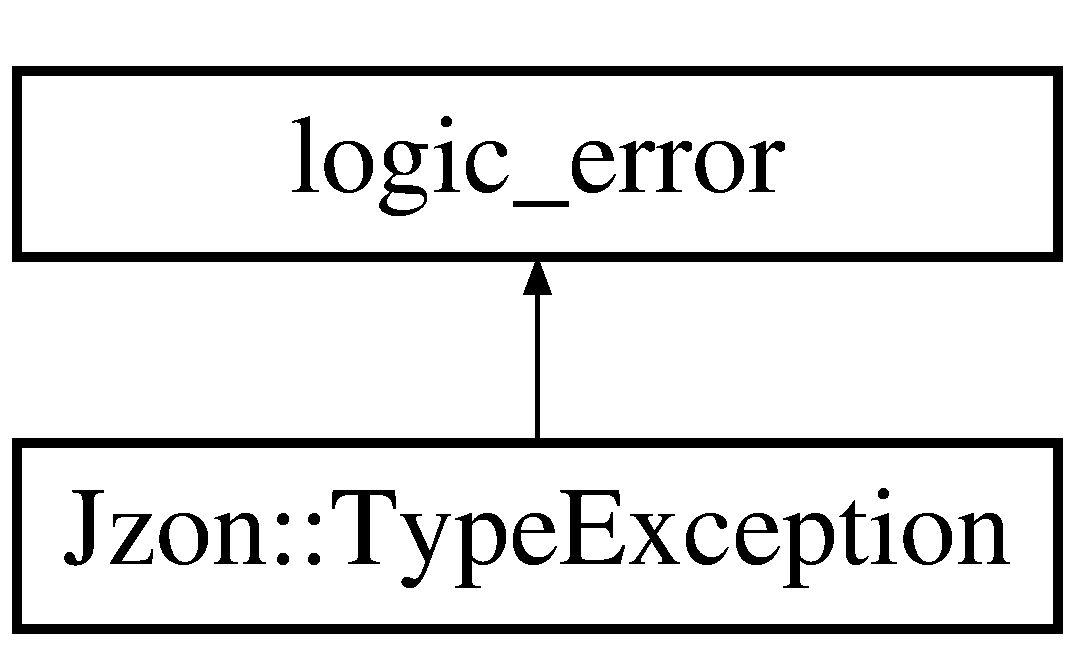
\includegraphics[height=2.000000cm]{class_jzon_1_1_type_exception}
\end{center}
\end{figure}


The documentation for this class was generated from the following file\-:\begin{DoxyCompactItemize}
\item 
Jzon.\-h\end{DoxyCompactItemize}

\hypertarget{class_unit}{\section{Unit Class Reference}
\label{class_unit}\index{Unit@{Unit}}
}
\subsection*{Public Member Functions}
\begin{DoxyCompactItemize}
\item 
\hypertarget{class_unit_ade0a34dce0fd220c0065959390de834b}{unsigned long {\bfseries give\-\_\-id} ()}\label{class_unit_ade0a34dce0fd220c0065959390de834b}

\end{DoxyCompactItemize}
\subsection*{Friends}
\begin{DoxyCompactItemize}
\item 
\hypertarget{class_unit_a2cedee6ab0da841755431efd84ad466b}{class {\bfseries Update}}\label{class_unit_a2cedee6ab0da841755431efd84ad466b}

\end{DoxyCompactItemize}


The documentation for this class was generated from the following file\-:\begin{DoxyCompactItemize}
\item 
Units.\-h\end{DoxyCompactItemize}

\hypertarget{class_update}{\section{Update Class Reference}
\label{class_update}\index{Update@{Update}}
}
\subsection*{Public Member Functions}
\begin{DoxyCompactItemize}
\item 
\hypertarget{class_update_a28dd7deebaa2863e30291986e70061bb}{{\bfseries Update} (string)}\label{class_update_a28dd7deebaa2863e30291986e70061bb}

\item 
\hypertarget{class_update_a8bb780249712a2b0fdcfa1450a65be75}{vector$<$ \hyperlink{class_player}{Player} $>$ $\ast$ {\bfseries get\-\_\-players} ()}\label{class_update_a8bb780249712a2b0fdcfa1450a65be75}

\item 
\hypertarget{class_update_abaebc1704b7c2b3abbba1ca5f20b58b5}{void {\bfseries main\-\_\-update} ()}\label{class_update_abaebc1704b7c2b3abbba1ca5f20b58b5}

\item 
\hypertarget{class_update_a20f41e11b35a3ff407ffadf8d33a5465}{void {\bfseries update\-\_\-units} (\hyperlink{class_orders}{Orders} \&)}\label{class_update_a20f41e11b35a3ff407ffadf8d33a5465}

\item 
\hypertarget{class_update_a68cffdaf2707f7c02e64c71d62b479a1}{void {\bfseries update\-\_\-buys} (map$<$ string, unsigned int $>$)}\label{class_update_a68cffdaf2707f7c02e64c71d62b479a1}

\item 
\hypertarget{class_update_a0ae8c95d836686436e19e15f7be3e043}{queue$<$ \hyperlink{class_orders}{Orders} $>$ {\bfseries get\-\_\-orders} ()}\label{class_update_a0ae8c95d836686436e19e15f7be3e043}

\item 
\hypertarget{class_update_a430086cc0eb5ac98b38776b576cff239}{bool {\bfseries has\-\_\-orders} ()}\label{class_update_a430086cc0eb5ac98b38776b576cff239}

\item 
\hypertarget{class_update_afa1e25b78b8a227b09235d894e0e2d33}{void {\bfseries add\-\_\-unit} (queue$<$ string $>$)}\label{class_update_afa1e25b78b8a227b09235d894e0e2d33}

\end{DoxyCompactItemize}
\subsection*{Friends}
\begin{DoxyCompactItemize}
\item 
\hypertarget{class_update_af90c3329e2433f8dce3ad0ae3b483cfe}{void {\bfseries tick\-\_\-function} (\hyperlink{struct_properties}{Properties} \&, \hyperlink{class_update}{Update} \&)}\label{class_update_af90c3329e2433f8dce3ad0ae3b483cfe}

\end{DoxyCompactItemize}


The documentation for this class was generated from the following file\-:\begin{DoxyCompactItemize}
\item 
Update.\-h\end{DoxyCompactItemize}

\hypertarget{class_jzon_1_1_value}{\section{Jzon\-:\-:Value Class Reference}
\label{class_jzon_1_1_value}\index{Jzon\-::\-Value@{Jzon\-::\-Value}}
}
Inheritance diagram for Jzon\-:\-:Value\-:\begin{figure}[H]
\begin{center}
\leavevmode
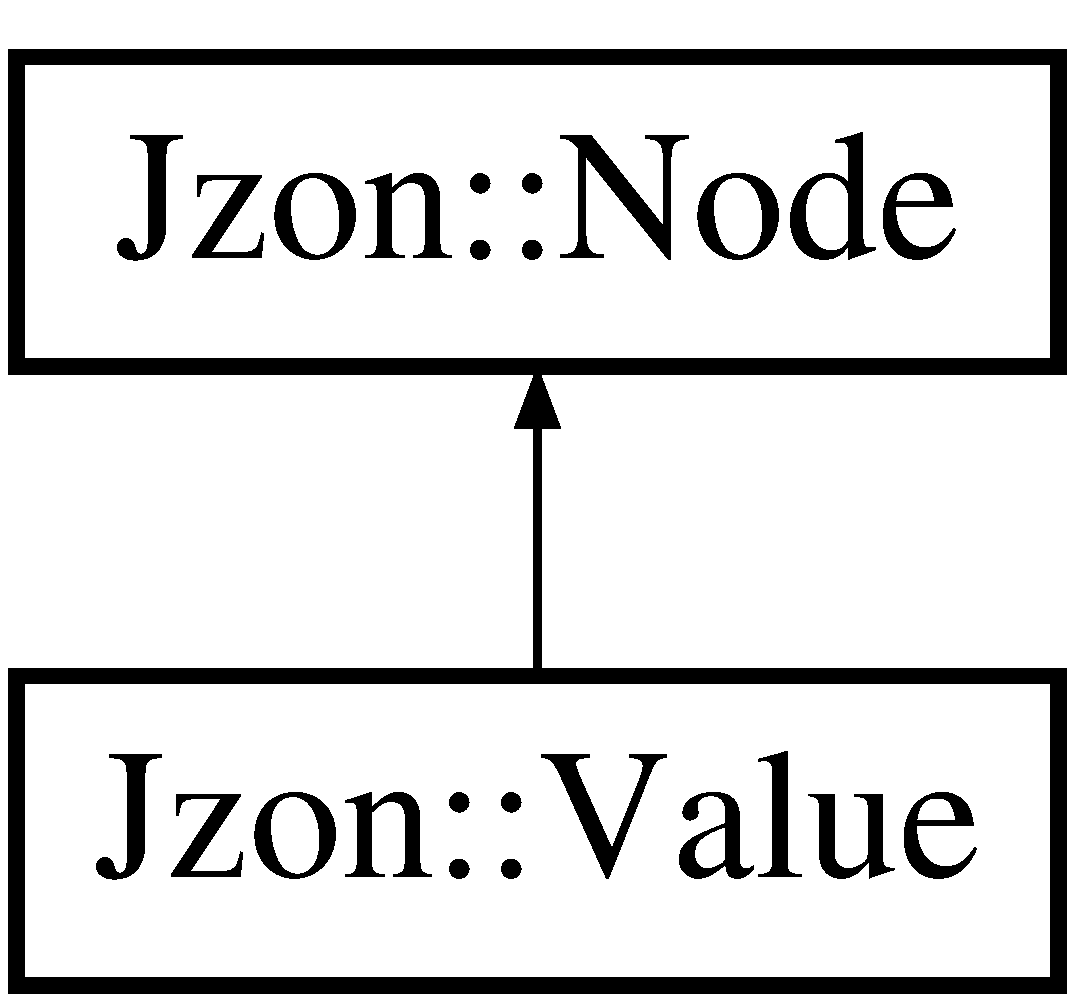
\includegraphics[height=2.000000cm]{class_jzon_1_1_value}
\end{center}
\end{figure}
\subsection*{Public Types}
\begin{DoxyCompactItemize}
\item 
enum {\bfseries Value\-Type} \{ {\bfseries V\-T\-\_\-\-N\-U\-L\-L}, 
{\bfseries V\-T\-\_\-\-S\-T\-R\-I\-N\-G}, 
{\bfseries V\-T\-\_\-\-N\-U\-M\-B\-E\-R}, 
{\bfseries V\-T\-\_\-\-B\-O\-O\-L}
 \}
\end{DoxyCompactItemize}
\subsection*{Public Member Functions}
\begin{DoxyCompactItemize}
\item 
\hypertarget{class_jzon_1_1_value_afad65ce426209f080d9457af440f7288}{{\bfseries Value} (const \hyperlink{class_jzon_1_1_value}{Value} \&rhs)}\label{class_jzon_1_1_value_afad65ce426209f080d9457af440f7288}

\item 
\hypertarget{class_jzon_1_1_value_a7647574ac67ba6b893e7cd1816478928}{{\bfseries Value} (const \hyperlink{class_jzon_1_1_node}{Node} \&rhs)}\label{class_jzon_1_1_value_a7647574ac67ba6b893e7cd1816478928}

\item 
\hypertarget{class_jzon_1_1_value_a96eb79fb74d4a58ba265768483687785}{{\bfseries Value} (Value\-Type type, const std\-::string \&value)}\label{class_jzon_1_1_value_a96eb79fb74d4a58ba265768483687785}

\item 
\hypertarget{class_jzon_1_1_value_acc14b12aaf5821945db6e66f51025aa0}{{\bfseries Value} (const std\-::string \&value)}\label{class_jzon_1_1_value_acc14b12aaf5821945db6e66f51025aa0}

\item 
\hypertarget{class_jzon_1_1_value_a50ad69707bebef4b26f708a4d0a272ce}{{\bfseries Value} (const char $\ast$value)}\label{class_jzon_1_1_value_a50ad69707bebef4b26f708a4d0a272ce}

\item 
\hypertarget{class_jzon_1_1_value_a0c20325c8d3b407ad4ec025e4f182b87}{{\bfseries Value} (const int value)}\label{class_jzon_1_1_value_a0c20325c8d3b407ad4ec025e4f182b87}

\item 
\hypertarget{class_jzon_1_1_value_a634fe3f4c85eb6fd1b205aaa1fe16f13}{{\bfseries Value} (const float value)}\label{class_jzon_1_1_value_a634fe3f4c85eb6fd1b205aaa1fe16f13}

\item 
\hypertarget{class_jzon_1_1_value_a6d3057edd2b44dd186b6d0626d642dc0}{{\bfseries Value} (const double value)}\label{class_jzon_1_1_value_a6d3057edd2b44dd186b6d0626d642dc0}

\item 
\hypertarget{class_jzon_1_1_value_a63139d2fe9ea9e19506497e6ee5a1aaf}{{\bfseries Value} (const bool value)}\label{class_jzon_1_1_value_a63139d2fe9ea9e19506497e6ee5a1aaf}

\item 
\hypertarget{class_jzon_1_1_value_a1befad9158be8b291868efaeacc6eb94}{virtual Type {\bfseries Get\-Type} () const }\label{class_jzon_1_1_value_a1befad9158be8b291868efaeacc6eb94}

\item 
\hypertarget{class_jzon_1_1_value_a9a5169042399033b49645438abf50dfa}{Value\-Type {\bfseries Get\-Value\-Type} () const }\label{class_jzon_1_1_value_a9a5169042399033b49645438abf50dfa}

\item 
\hypertarget{class_jzon_1_1_value_aad023cb9365b877b697321298f19fc3f}{virtual bool {\bfseries Is\-Null} () const }\label{class_jzon_1_1_value_aad023cb9365b877b697321298f19fc3f}

\item 
\hypertarget{class_jzon_1_1_value_a36aab3d04072f66b4bc06d5b16da3234}{virtual bool {\bfseries Is\-String} () const }\label{class_jzon_1_1_value_a36aab3d04072f66b4bc06d5b16da3234}

\item 
\hypertarget{class_jzon_1_1_value_a1a33452554cbef750ba7d6c354ee3478}{virtual bool {\bfseries Is\-Number} () const }\label{class_jzon_1_1_value_a1a33452554cbef750ba7d6c354ee3478}

\item 
\hypertarget{class_jzon_1_1_value_ac32759b1ddc718d5d11a94ad11deff95}{virtual bool {\bfseries Is\-Bool} () const }\label{class_jzon_1_1_value_ac32759b1ddc718d5d11a94ad11deff95}

\item 
\hypertarget{class_jzon_1_1_value_af70e83ee3cf2f1bb6ea07dc098160d3d}{virtual std\-::string {\bfseries To\-String} () const }\label{class_jzon_1_1_value_af70e83ee3cf2f1bb6ea07dc098160d3d}

\item 
\hypertarget{class_jzon_1_1_value_adbb4d6bdc55bb4fe44932c6138ceba5f}{virtual int {\bfseries To\-Int} () const }\label{class_jzon_1_1_value_adbb4d6bdc55bb4fe44932c6138ceba5f}

\item 
\hypertarget{class_jzon_1_1_value_aca0a22646cb02d8dcc6a6e2433203d9d}{virtual float {\bfseries To\-Float} () const }\label{class_jzon_1_1_value_aca0a22646cb02d8dcc6a6e2433203d9d}

\item 
\hypertarget{class_jzon_1_1_value_a313147446f7c3b1ee70b63fc811fcdb0}{virtual double {\bfseries To\-Double} () const }\label{class_jzon_1_1_value_a313147446f7c3b1ee70b63fc811fcdb0}

\item 
\hypertarget{class_jzon_1_1_value_ad56b42fc1d156dded80060674b2fed71}{virtual bool {\bfseries To\-Bool} () const }\label{class_jzon_1_1_value_ad56b42fc1d156dded80060674b2fed71}

\item 
\hypertarget{class_jzon_1_1_value_ac15339ae6c02c936537b7c543a282e21}{void {\bfseries Set\-Null} ()}\label{class_jzon_1_1_value_ac15339ae6c02c936537b7c543a282e21}

\item 
\hypertarget{class_jzon_1_1_value_afe8d653c1ba5a11e4bb3f0973df8addc}{void {\bfseries Set} (const \hyperlink{class_jzon_1_1_value}{Value} \&value)}\label{class_jzon_1_1_value_afe8d653c1ba5a11e4bb3f0973df8addc}

\item 
\hypertarget{class_jzon_1_1_value_a78f9cf22b6e2944dd9c8029df5a0caa0}{void {\bfseries Set} (Value\-Type type, const std\-::string \&value)}\label{class_jzon_1_1_value_a78f9cf22b6e2944dd9c8029df5a0caa0}

\item 
\hypertarget{class_jzon_1_1_value_ac92a676958ef33a7ec22f6c8f83b1a99}{void {\bfseries Set} (const std\-::string \&value)}\label{class_jzon_1_1_value_ac92a676958ef33a7ec22f6c8f83b1a99}

\item 
\hypertarget{class_jzon_1_1_value_aa144e4f5908b85fb0cbd58550e1fb814}{void {\bfseries Set} (const char $\ast$value)}\label{class_jzon_1_1_value_aa144e4f5908b85fb0cbd58550e1fb814}

\item 
\hypertarget{class_jzon_1_1_value_a371577c1b6829c4313287264e6effaed}{void {\bfseries Set} (const int value)}\label{class_jzon_1_1_value_a371577c1b6829c4313287264e6effaed}

\item 
\hypertarget{class_jzon_1_1_value_a1b4746098fa6f7e082c7d619e47ead6c}{void {\bfseries Set} (const float value)}\label{class_jzon_1_1_value_a1b4746098fa6f7e082c7d619e47ead6c}

\item 
\hypertarget{class_jzon_1_1_value_a900250dc37d85e531cd8be31bd282287}{void {\bfseries Set} (const double value)}\label{class_jzon_1_1_value_a900250dc37d85e531cd8be31bd282287}

\item 
\hypertarget{class_jzon_1_1_value_a39df6bbd7512e4ea7ae3497528322a70}{void {\bfseries Set} (const bool value)}\label{class_jzon_1_1_value_a39df6bbd7512e4ea7ae3497528322a70}

\item 
\hypertarget{class_jzon_1_1_value_ab42a29c2348be769558d9f4fd32e49d9}{\hyperlink{class_jzon_1_1_value}{Value} \& {\bfseries operator=} (const \hyperlink{class_jzon_1_1_value}{Value} \&rhs)}\label{class_jzon_1_1_value_ab42a29c2348be769558d9f4fd32e49d9}

\item 
\hypertarget{class_jzon_1_1_value_a9ccb8336d77c1b73a2e79b35e57ecf96}{\hyperlink{class_jzon_1_1_value}{Value} \& {\bfseries operator=} (const \hyperlink{class_jzon_1_1_node}{Node} \&rhs)}\label{class_jzon_1_1_value_a9ccb8336d77c1b73a2e79b35e57ecf96}

\item 
\hypertarget{class_jzon_1_1_value_aad6d4b101c9c066827e0dfbb664c4fd1}{\hyperlink{class_jzon_1_1_value}{Value} \& {\bfseries operator=} (const std\-::string \&rhs)}\label{class_jzon_1_1_value_aad6d4b101c9c066827e0dfbb664c4fd1}

\item 
\hypertarget{class_jzon_1_1_value_a82687c3b9cf55d5b181dfc4db05bc3be}{\hyperlink{class_jzon_1_1_value}{Value} \& {\bfseries operator=} (const char $\ast$rhs)}\label{class_jzon_1_1_value_a82687c3b9cf55d5b181dfc4db05bc3be}

\item 
\hypertarget{class_jzon_1_1_value_a745c6eda32d25bbbc0ad3c61bc6b9142}{\hyperlink{class_jzon_1_1_value}{Value} \& {\bfseries operator=} (const int rhs)}\label{class_jzon_1_1_value_a745c6eda32d25bbbc0ad3c61bc6b9142}

\item 
\hypertarget{class_jzon_1_1_value_a3975a602470745d6740a1fac6bad8464}{\hyperlink{class_jzon_1_1_value}{Value} \& {\bfseries operator=} (const float rhs)}\label{class_jzon_1_1_value_a3975a602470745d6740a1fac6bad8464}

\item 
\hypertarget{class_jzon_1_1_value_ae5dadcd905d3fa88d52e54508e1f5304}{\hyperlink{class_jzon_1_1_value}{Value} \& {\bfseries operator=} (const double rhs)}\label{class_jzon_1_1_value_ae5dadcd905d3fa88d52e54508e1f5304}

\item 
\hypertarget{class_jzon_1_1_value_aaf37b358090dbcf97636fd18541888d8}{\hyperlink{class_jzon_1_1_value}{Value} \& {\bfseries operator=} (const bool rhs)}\label{class_jzon_1_1_value_aaf37b358090dbcf97636fd18541888d8}

\item 
\hypertarget{class_jzon_1_1_value_aacc445598e286eca43a6f7abc75754c0}{bool {\bfseries operator==} (const \hyperlink{class_jzon_1_1_value}{Value} \&other) const }\label{class_jzon_1_1_value_aacc445598e286eca43a6f7abc75754c0}

\item 
\hypertarget{class_jzon_1_1_value_a6f626502ac2e99b3c3a7adceb03ac04f}{bool {\bfseries operator!=} (const \hyperlink{class_jzon_1_1_value}{Value} \&other) const }\label{class_jzon_1_1_value_a6f626502ac2e99b3c3a7adceb03ac04f}

\end{DoxyCompactItemize}
\subsection*{Static Public Member Functions}
\begin{DoxyCompactItemize}
\item 
\hypertarget{class_jzon_1_1_value_a8530bdf0704914e5fd04736fcb79916a}{static std\-::string {\bfseries Escape\-String} (const std\-::string \&value)}\label{class_jzon_1_1_value_a8530bdf0704914e5fd04736fcb79916a}

\item 
\hypertarget{class_jzon_1_1_value_a5207673a51de4ebd9c9e39b1f121634b}{static std\-::string {\bfseries Unescape\-String} (const std\-::string \&value)}\label{class_jzon_1_1_value_a5207673a51de4ebd9c9e39b1f121634b}

\end{DoxyCompactItemize}
\subsection*{Protected Member Functions}
\begin{DoxyCompactItemize}
\item 
\hypertarget{class_jzon_1_1_value_af5b4f128f89c0d63fddf0bd5deb83860}{virtual \hyperlink{class_jzon_1_1_node}{Node} $\ast$ {\bfseries Get\-Copy} () const }\label{class_jzon_1_1_value_af5b4f128f89c0d63fddf0bd5deb83860}

\end{DoxyCompactItemize}


The documentation for this class was generated from the following files\-:\begin{DoxyCompactItemize}
\item 
Jzon.\-h\item 
Jzon.\-cpp\end{DoxyCompactItemize}

\hypertarget{class_jzon_1_1_value_exception}{\section{Jzon\-:\-:Value\-Exception Class Reference}
\label{class_jzon_1_1_value_exception}\index{Jzon\-::\-Value\-Exception@{Jzon\-::\-Value\-Exception}}
}
Inheritance diagram for Jzon\-:\-:Value\-Exception\-:\begin{figure}[H]
\begin{center}
\leavevmode
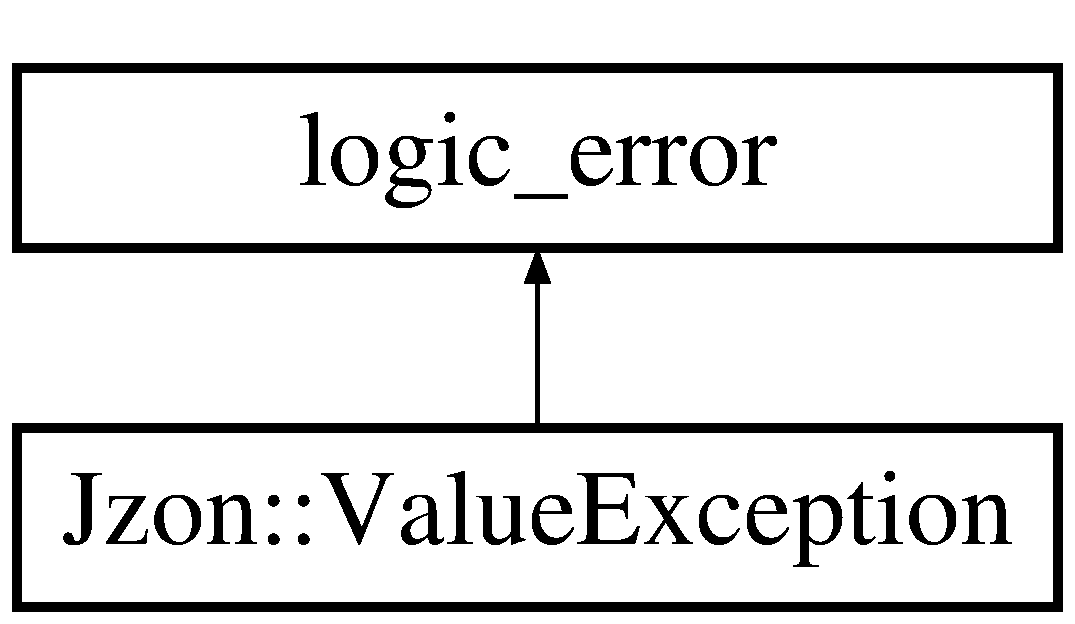
\includegraphics[height=2.000000cm]{class_jzon_1_1_value_exception}
\end{center}
\end{figure}


The documentation for this class was generated from the following file\-:\begin{DoxyCompactItemize}
\item 
Jzon.\-h\end{DoxyCompactItemize}

\hypertarget{class_jzon_1_1_writer}{\section{Jzon\-:\-:Writer Class Reference}
\label{class_jzon_1_1_writer}\index{Jzon\-::\-Writer@{Jzon\-::\-Writer}}
}
\subsection*{Public Member Functions}
\begin{DoxyCompactItemize}
\item 
\hypertarget{class_jzon_1_1_writer_a149d7419887f854a3b480194632f5bd3}{{\bfseries Writer} (const \hyperlink{class_jzon_1_1_node}{Node} \&root, const \hyperlink{struct_jzon_1_1_format}{Format} \&format=No\-Format)}\label{class_jzon_1_1_writer_a149d7419887f854a3b480194632f5bd3}

\item 
\hypertarget{class_jzon_1_1_writer_a2551d27b952fbd2f8bf9c1e9003c27e6}{{\bfseries Writer} (const \hyperlink{class_jzon_1_1_node}{Node} \&root, const std\-::string \&filename, const \hyperlink{struct_jzon_1_1_format}{Format} \&format=No\-Format)}\label{class_jzon_1_1_writer_a2551d27b952fbd2f8bf9c1e9003c27e6}

\item 
\hypertarget{class_jzon_1_1_writer_a260fcff96207b12dd1a99b2482879247}{void {\bfseries Set\-Filename} (const std\-::string \&filename)}\label{class_jzon_1_1_writer_a260fcff96207b12dd1a99b2482879247}

\item 
\hypertarget{class_jzon_1_1_writer_a07f8479fa59920d8e3223e17d087918b}{void {\bfseries Set\-Format} (const \hyperlink{struct_jzon_1_1_format}{Format} \&format)}\label{class_jzon_1_1_writer_a07f8479fa59920d8e3223e17d087918b}

\item 
\hypertarget{class_jzon_1_1_writer_a592006df4de2c148f6dc629c8e01ea77}{void {\bfseries Write} ()}\label{class_jzon_1_1_writer_a592006df4de2c148f6dc629c8e01ea77}

\item 
\hypertarget{class_jzon_1_1_writer_a6200aa0421736ab18a8d1ecdb4dae597}{const std\-::string \& {\bfseries Get\-Result} () const }\label{class_jzon_1_1_writer_a6200aa0421736ab18a8d1ecdb4dae597}

\end{DoxyCompactItemize}


The documentation for this class was generated from the following files\-:\begin{DoxyCompactItemize}
\item 
Jzon.\-h\item 
Jzon.\-cpp\end{DoxyCompactItemize}

\chapter{File Documentation}
\hypertarget{rules_8cpp}{\section{rules.\-cpp File Reference}
\label{rules_8cpp}\index{rules.\-cpp@{rules.\-cpp}}
}
{\ttfamily \#include \char`\"{}rules.\-h\char`\"{}}\\*

\hypertarget{rules_8h}{\section{rules.\-h File Reference}
\label{rules_8h}\index{rules.\-h@{rules.\-h}}
}
{\ttfamily \#include $<$map$>$}\\*
{\ttfamily \#include $<$string$>$}\\*
{\ttfamily \#include $<$vector$>$}\\*
{\ttfamily \#include $<$sstream$>$}\\*
{\ttfamily \#include $<$list$>$}\\*
{\ttfamily \#include $<$set$>$}\\*
{\ttfamily \#include $<$iostream$>$}\\*
{\ttfamily \#include $<$fstream$>$}\\*
{\ttfamily \#include \char`\"{}Jzon.\-h\char`\"{}}\\*
\subsection*{Classes}
\begin{DoxyCompactItemize}
\item 
class \hyperlink{class_rules_1_1_rules_entry}{Rules\-::\-Rules\-Entry}
\begin{DoxyCompactList}\small\item\em Data structure for individual rules entries. \end{DoxyCompactList}\item 
class \hyperlink{class_rules_1_1_rules_container}{Rules\-::\-Rules\-Container}
\begin{DoxyCompactList}\small\item\em Parent container for game rules. \end{DoxyCompactList}\end{DoxyCompactItemize}

\addcontentsline{toc}{part}{Index}
\printindex
\end{document}
